% Version 3.1 December 2024
% See section 11 of the User Manual for version history
%
%%%%%%%%%%%%%%%%%%%%%%%%%%%%%%%%%%%%%%%%%%%%%%%%%%%%%%%%%%%%%%%%%%%%%%
%%                                                                 %%
%% Please do not use \input{...} to include other tex files.       %%
%% Submit your LaTeX manuscript as one .tex document.              %%
%%                                                                 %%
%% All additional figures and files should be attached             %%
%% separately and not embedded in the \TeX\ document itself.       %%
%%                                                                 %%
%%%%%%%%%%%%%%%%%%%%%%%%%%%%%%%%%%%%%%%%%%%%%%%%%%%%%%%%%%%%%%%%%%%%%

%%\documentclass[referee,sn-basic]{sn-jnl}% referee option is meant for double line spacing

%%=======================================================%%
%% to print line numbers in the margin use lineno option %%
%%=======================================================%%

%%\documentclass[lineno,pdflatex,sn-basic]{sn-jnl}% Basic Springer Nature Reference Style/Chemistry Reference Style

%%=========================================================================================%%
%% the documentclass is set to pdflatex as default. You can delete it if not appropriate.  %%
%%=========================================================================================%%

%%\documentclass[sn-basic]{sn-jnl}% Basic Springer Nature Reference Style/Chemistry Reference Style

%%Note: the following reference styles support Namedate and Numbered referencing. By default the style follows the most common style. To switch between the options you can add or remove “Numbered” in the optional parenthesis. 
%%The option is available for: sn-basic.bst, sn-chicago.bst%  
 
%%\documentclass[pdflatex,sn-nature]{sn-jnl}% Style for submissions to Nature Portfolio journals
%%\documentclass[pdflatex,sn-basic]{sn-jnl}% Basic Springer Nature Reference Style/Chemistry Reference Style
\documentclass[pdflatex,sn-mathphys-num, oneside, 11pt]{sn-jnl}% Math and Physical Sciences Numbered Reference Style
%%\documentclass[pdflatex,sn-mathphys-ay]{sn-jnl}% Math and Physical Sciences Author Year Reference Style
%%\documentclass[pdflatex,sn-aps]{sn-jnl}% American Physical Society (APS) Reference Style
%%\documentclass[pdflatex,sn-vancouver-num]{sn-jnl}% Vancouver Numbered Reference Style
%%\documentclass[pdflatex,sn-vancouver-ay]{sn-jnl}% Vancouver Author Year Reference Style
%%\documentclass[pdflatex,sn-apa]{sn-jnl}% APA Reference Style
%%\documentclass[pdflatex,sn-chicago]{sn-jnl}% Chicago-based Humanities Reference Style

%%%% Standard Packages
%%<additional latex packages if required can be included here>

\usepackage{float}
\usepackage{gensymb}
\usepackage{graphicx}%
\usepackage{multirow}%
\usepackage{amsmath,amssymb,amsfonts}%
\usepackage{amsthm}%
\usepackage{mathrsfs}%
\usepackage[title]{appendix}%
\usepackage{xcolor}%
\usepackage{textcomp}%
\usepackage{manyfoot}%
\usepackage{booktabs}%
\usepackage{algorithm}%
\usepackage{algorithmicx}%
\usepackage{algpseudocode}%
\usepackage{listings}%
\usepackage{geometry}
\geometry{
  reset,          
  a4paper,
  textwidth=190mm,% Forces the text width (A4 is 210mm wide - 10L - 10R = 190mm)
  textheight=267mm, % Forces the text height (A4 is 297mm tall - 15T - 15B = 267mm)
  left=10mm,
  right=10mm,
  top=15mm,
  bottom=18mm
}
%%%%

%%%%%=============================================================================%%%%
%%%%  Remarks: This template is provided to aid authors with the preparation
%%%%  of original research articles intended for submission to journals published 
%%%%  by Springer Nature. The guidance has been prepared in partnership with 
%%%%  production teams to conform to Springer Nature technical requirements. 
%%%%  Editorial and presentation requirements differ among journal portfolios and 
%%%%  research disciplines. You may find sections in this template are irrelevant 
%%%%  to your work and are empowered to omit any such section if allowed by the 
%%%%  journal you intend to submit to. The submission guidelines and policies 
%%%%  of the journal take precedence. A detailed User Manual is available in the 
%%%%  template package for technical guidance.
%%%%%=============================================================================%%%%

%% as per the requirement new theorem styles can be included as shown below
\theoremstyle{thmstyleone}%
\newtheorem{theorem}{Theorem}%  meant for continuous numbers
%%\newtheorem{theorem}{Theorem}[section]% meant for sectionwise numbers
%% optional argument [theorem] produces theorem numbering sequence instead of independent numbers for Proposition
\newtheorem{proposition}[theorem]{Proposition}% 
%%\newtheorem{proposition}{Proposition}% to get separate numbers for theorem and proposition etc.

\theoremstyle{thmstyletwo}%
\newtheorem{example}{Example}%
\newtheorem{remark}{Remark}%

\theoremstyle{thmstylethree}%
\newtheorem{definition}{Definition}%

\raggedbottom
%%\unnumbered% uncomment this for unnumbered level heads

% - NEW SPACE-SAVING COMMANDS -
\usepackage{microtype}      % 1. Optimizes horizontal text packing (Saves ~5% space)
\linespread{0.96}           % 2. Reduces vertical space between lines (Saves ~5% space)
\usepackage{newtxtext}      % 3. Ensures you are using the most modern, compact Times font
\usepackage{newtxmath}
% ---------

\begin{document}

\title[Article Title]{Are meteorological, agricultural, and satellite features from the CY-Bench Dataset good predictors of European Wheat Futures Price Changes?}

%%=============================================================%%
%% GivenName	-> \fnm{Joergen W.}
%% Particle	-> \spfx{van der} -> surname prefix
%% FamilyName	-> \sur{Ploeg}
%% Suffix	-> \sfx{IV}
%% \author*[1,2]{\fnm{Joergen W.} \spfx{van der} \sur{Ploeg} 
%%  \sfx{IV}}\email{iauthor@gmail.com}
%%=============================================================%%

\author{\fnm{68729}}
\author{\fnm{candidate number}}
\author{\fnm{candidate number}}

%%\pacs[JEL Classification]{D8, H51}

%%\pacs[MSC Classification]{35A01, 65L10, 65L12, 65L20, 65L70}

\maketitle

\clearpage

\section{Executive Summary}\label{execsum}

\clearpage

\section{Table of Contents}\label{contents}

\clearpage

\section{Introduction (1 page)}\label{intro}

\clearpage

\section{(Optional) Literature Review (1 page)}\label{lit_review}

There are two sets of research topics that motivate our literature review: the application of machine learning to multi-national crop yield forecasting, and the use of data-driven models to forecast wheat futures using agricultural signals as inputs. Both areas of research have developed substantially in recent years, but largely in parallel, with limited work connecting yield forecasting outputs to commodity price models. The review below covers both sets of papers.\\
 
We start with the foundations of ML-based crop yield prediction as described by van Klompenburg, Kassahun, and Catal~\cite{bib14}, who conducted a systematic literature review of 50 studies across a range of crops, algorithms, and geographies. The feature sets and model choices most commonly adopted were temperature, rainfall, and soil type as the dominant predictors. In terms of model selection, their review found that no single model emerged as definitively best, but that Random Forest, Neural Networks, Linear Regression, and Gradient Boosting were the most frequently used, with most studies testing a variety of models to identify the best performer for their specific task. The most widely used evaluation method was 10-fold cross-validation, and artificial neural networks were the most widely applied model class. They also looked at deep learning literature and found CNNs, LSTMs, and DNNs to be the core architectures for this prediction task. Importantly, their review highlighted data availability as the primary constraint on generalization. They found that studies were typically operated over limited geographic extents with short time series, making it difficult to draw conclusions about which methods transfer across regions or climates. Oikonomidis, Catal, and Kassahun~\cite{bib15} extended the ML crop yield review specifically to deep learning approaches, systematically analysing 44 primary studies. Their results confirmed CNN as both the most frequently applied deep learning algorithm and the best-performing one across studies, with LSTM and DNN following as the next most common architectures. They found that RMSE was the dominant evaluation metric used across the reviewed literature. Crucially, they also found that the most significant challenge was the limitation of large training datasets due to insufficient data availability. This raised the risk of overfitting and reduced real-world model performance, with proposed solutions including data augmentation and transfer learning. This data constraint is consistent with what van Klompenburg et al.~\cite{bib14} identified in their ML literature as the primary constraint, so together the two reviews establish data availability and geographic coverage as the primary bottleneck to building generalisable crop yield prediction models. Muruganantham et al.~\cite{bib20} conducted a further systematic review specifically combining deep learning with remote sensing for crop yield prediction, analysing 44 studies from 2012 to 2022 and confirming the previous findings that LSTM and CNN are the dominant approaches, with satellite-derived vegetation indices emerging as among the most informative input features alongside weather variables.\\
 
Paudel et al.~\cite{bib16} attempt to address these gaps by establishing a large-scale ML baseline for crop yield prediction across multiple countries and crop types. Working with a feature set covering meteorological variables, crop model outputs, and remote sensing indicators, they evaluated Ridge Regression, KNN, SVM, and Gradient Boosting under a time-based look-forward cross-validation scheme that simulates operational forecasting conditions by training only on data preceding each test year on 70 percent train, 30 percent test split. They looked at three European countries, the Netherlands, Germany, and France, evaluating five crop types, with predictions made at the regional level and then aggregated to the national level for comparison with the established European Commission’s "Monitoring Agricultural ResourceS Crop Yield Forecasting System" (MCYFS). Their results showed that early-season predictions made 30 days after planting were broadly competitive with the MCYFS in most cases. They note that accuracy improved as the season progressed toward harvest, confirming that lead time is a key constraint for any real-time application.\\
 
The most recent CY-Bench paper Paudel et al.~\cite{bib17} built on this foundation at a global scale, combining predictor data, including meteorological variables such as temperature, precipitation, evapotranspiration, and solar radiation, with soil data like available water capacity, bulk density, drainage class, and moisture content. Lastly, they also used satellite vegetation across 29 wheat-growing and 42 maize-growing countries. For features, the dataset includes threshold-based indicators such as counts of cold days, hot days, and dry days during the growing season, for the purpose of tracking climate-related stress signals on the crops. Model evaluation uses Leave One Year Out cross-validation to obtain estimates of performance across both typical and extreme harvest years, with normalized root mean squared error and mean absolute percentage error as the primary metrics to support cross-country comparison. Baseline models evaluated include Ridge Regression, Random Forest, and LSTM, which were all compared against a Naive Average Yield benchmark. These two Paudel studies together define the current benchmark results for the CY-Bench dataset for crop yield forecasting.\\
 
In terms of modelling agricultural commodity price dynamics, Theofilou et al.~\cite{bib21} provide a systematic review of 50 Machine Learning studies applied to wheat, corn, and rice price forecasting, finding that hybrid deep learning models consistently outperform traditional approaches (such as ARIMA and Partial Least Squares Regression), and identifying persistent challenges including reliance on region-specific datasets and limited model interpretability. Li~\cite{bib18} benchmarks Holt-Winters exponential smoothing against three LSTM-based variants on a European wheat spot price series, with the CNN-LSTM model achieving the best performance due to its ability to capture long-term dependencies and price trend characteristics. Zhang and Tang~\cite{bib22} propose a hybrid LSTM model where they decompose the agricultural commodity futures price time series into multiple smoother components (also called variational mode decomposition), finding that decomposition-based preprocessing substantially improves accuracy for volatile price series. Brignoli et al.~\cite{bib23} compare LSTM-RNNs against classical econometric models for grain futures price forecasting, finding that LSTM-RNNs consistently outperform at longer forecast horizons and are particularly capable of handling structural breaks in price series. They note specific challenges in handling seasonality and trends requiring extra pre-processing steps to remove these factors. Thaker, Chan, and Sonner~\cite{bib19} take a fundamentally different approach that bridges the yield and price literatures directly since they apply a CNN to aerial imagery of winter hard red wheat planted areas. They use cloud coverage patterns as a weather proxy for field-level yield conditions, and then train the model on this imagery to produce a 20 trading-day forecast for wheat futures price on the Chicago Mercantile Exchange with purely directional long or short trading recommendations. Their paper demonstrates that satellite-derived signals can generate positive alpha in wheat futures, but they also document performance decay once the signal becomes widely available. This is, again, a natural and expected limitation of this type of prediction task, potentially showing that the informational advantage of agricultural based price forecasts depend on signal differentiation from other traders.\\
 
Together, the reviewed literature establishes a clear gap. Indeed, the yield prediction task has produced well-validated, multi-national, in-season yield forecasts but has not connected these directly to commodity futures price modelling. Secondly, the literature on the price modelling task demonstrates the growing effectiveness of deep learning and hybrid models for agricultural price forecasting, but these approaches tend to focus on price history and market signals rather than on benchmarked yield predictors. Finally, Thaker et al.~\cite{bib19} come closest to bridging this gap by using satellite-derived yield proxies as price signals, however, they mainly rely on unvalidated aerial imagery rather than more established predictors. Our study attempts to address this gap by using CY-Bench yield predictors as structured fundamental inputs to a wheat futures price model.\\

\section{Data Preparation}\label{sec:dataprep}

This next section describes how we prepare the CY-Bench dataset for two distinct prediction tasks, namely, European Wheat Futures Prediction and Yield Prediction prior to harvest. We start by describing the preparation steps shared by both prediction tasks, namely the agricultural data and the daily harmonisation via last-observation-carried-forward interpolation. Secondly, we describe the wheat futures roll-adjusted data preparation justifying our key choices. Thirdly, we cover the two distinct region filtering choices we applied to the futures price prediction dataset as well as the yield prediction dataset. Finally, we obtain two datasets from the same underlying CY-Bench source: a daily-frequency panel for the wheat futures return prediction task (Section~\ref{subsec:futures_prep}), and an annual cross-section for the crop yield forecasting task (Section~\ref{subsec:yield_prep}).

\subsection{Agricultural Data and Daily Harmonisation}

Firstly, our agricultural data is taken from the CY-Bench dataset~\cite{bib17}, which provides sub-national time series of climate, soil, and vegetation variables for 29 wheat growing countries (although more crops are covered too). We restrict our analysis to France, Germany, and Poland totalling over 500 regions. We select these three countries for two reasons. First, they are the three largest wheat-producing EU member states, collectively accounting for approximately 43\% of total EU wheat output~\cite{bib28} and they are, therefore, the countries whose supply conditions are most likely to influence the Euronext Milling Wheat contract that serves as our prediction target. Second, France and Germany appear in the Paudel et~al.~\cite{bib16} benchmark study, providing established yield forecasting results against which we can validate our secondary task. For each region, CY-Bench has five categories of predictor variables which are kept at their native temporal resolutions. Meteorological variables from the AgERA5 reanalysis dataset~\cite{bib_boogaard2022} include daily minimum and maximum temperature (\textdegree C), precipitation flux (mm), and solar radiation flux (J\,m$^{-2}$). Further, we have Soil moisture indicators from the NASA Global Land Data Assimilation System (GLDAS)~\cite{bib_rodell2004} provide daily surface and root-zone soil moisture (kg\,m$^{-2}$), these capture the water available to crops below the surface. Additionally, Satellite-derived vegetation indices comprise two variables that measure crop health from space. The Normalised Difference Vegetation Index (NDVI), sourced from the MODIS sensor at 8-day resolution, quantifies how green and photosynthetically active the land surface is by comparing the reflectance of visible red light (which healthy vegetation absorbs) with near-infrared light (which it reflects); values range from $-1$ to $1$, with higher values indicating denser, healthier vegetation~\cite{bib_vermote2015}. The second satellite derived indice is the Fraction of Absorbed Photosynthetically Active Radiation (fPAR), sourced from the JRC at dekadal (approximately 10-day) resolution, measures the share of incoming sunlight in the wavelengths used for photosynthesis (400-700\,nm) that is actually absorbed by the crop canopy, expressed as a percentage~\cite{bib_seguini}. NDVI is an indirect proxy for vegetation vigour based on spectral reflectance and fPAR directly estimates how much solar energy the crop is capturing for growth, this makes the two variables complementary indicators of crop condition by nature.\\

We then create our features from these climate variables which all have different temporal resolutions we must harmonise the data so as to avoid data leakage. Here we choose to simply retain these frequencies and expand them to daily increments per region using last-observation-carried-forward (LOCF) interpolation, i.e. we fill each day with the most recently past observed value. LOCF is a standard approach in time series data imputation, however, by assuming the data is constant, it evidently introduces bias. Here, we specifically choose this method to simulate a real operational context in which we may not have access to the variables' true value. After this procedure, each region has a consistent set of variables aligned to a common daily calendar.\\

Finally, we note that the agricultural data's availability starts at different periods for different features, for instance, meteorological data starts in 01-01-2001 while soil data start 01-02-2003. Thus, we decide to start our dataset when GLDAS soil moisture data becomes available in February 2003~\cite{bib17} to ensure full data availability. Further, we ensure that our dataset finishes at the last observation for which all data agricultural variables are available, fPAR's last data point is on the 21-12-2023 which is the earliest of all variables, thus, our dataset ends on that day. Further details are later discussed in Section ~\ref{sec:feature_eng} for the scope of the yield prediction dataset.

\subsection{Futures Price Data from Bloomberg}

Secondly, our target variable data for the futures price prediction task is the Euronext Milling Wheat roll-adjusted daily closing prices obtained from Bloomberg for the period 01-02-2003 to 21-12-2023 (to align with our agricultural data), yielding 5,362 trading days. More precisely, we define the raw target data as the closing price of the earliest maturing Euronext Milling Wheat Futures Contract. This is because near-term futures contracts are usually most liquid as per Ripple and Moosa ~\cite{bib84}. We use Bloomberg's ratio roll-adjustment to the time series $10$ days before each contract expiry, this means that historical prices are multiplied by $P_{new \ contract} / P_{old \ contract}$ so as to preserve the percentage returns across all rolls. Our choice of $10$ days before expiry is due to liquidity factors, indeed, futures contract generally decrease in liquidity as they get closer to maturity as per Ding and Lim~\cite{bib26}. Further, Carchano and Pardo's~\cite{bib25} study of stock index futures shows that choice of rollover timing does not induce statistically significant differences between the resulting return series. However, their study focuses on stock index futures rather than agricultural commodities which may exhibit stronger maturity effects due to seasonal supply factors. As per L{\'o}pez de Prado Chapter~2 ~\cite{bib24}, roll-adjustment is a key step as it eliminates the artificial jumps that occur at expiration to preserve the return dynamics experienced by a roll-following investor. This property is directly relevant to our study because the prediction target is a percentage return, not an absolute price level. A limitation of ratio adjustment is that it distorts historical price \emph{levels} (early-period prices may become very small or very large), making the series unsuitable for level-based analysis; however, since we use only returns and return-derived features, this limitation does not affect our study.

We retain two key fields from the raw data, closing price as well as volume. We note that while price has no missing data, missing volume data is forward-filled using LOCF. In this case, the missing volume data represents only 290 trading days or c.5.4\% of trading days.

\subsection{Region filtering and excluded areas}

Lastly, we detail our region filtering steps for the futures price prediction task where we exclude urban/non-wheat producing regions and then for the yield prediction task where we exclude regions with significant missing yield data due to lack of reporting.\\

Looking at the futures prediction task, When creating our agricultural features we exclude some highly urban and non-wheat producing regions as they should not directly be influencing the supply of wheat. We implement this simply filtering regions that are not included within CY-bench's raw yield data. Indeed, as per our \autoref{tab:region_classification} in the Appendix, we see that these regions are either urban, logistic hubs or non-wheat producing. This means that we retain 507 regions across France (94 regions), Germany (396 regions), and Poland (17 regions) (out of 518). \\

For the yield forecasting task, we apply a different region filter. Indeed, we retain only the 357 regions (90 French, 251 German, 16 Polish) that report wheat yield statistics for every year in the 2003 to 2020 window. The start year is the same as the futures prediction task dataset i.e. the start of the GLDAS soil moisture data. However, the end year is constrained by the latest available sub-national yield statistics from the JRC harmonised European dataset~\cite{bib_ronchetti2024}, which provides French and Polish NUTS-level yields through 2020. Although these filters lead to some information loss, it is not material. The 357 retained regions account for 97.5\% of total wheat production across the three countries (99.9\% for France, 93.3\% for Germany, 99.4\% for Poland). Indeed, the dropped regions are predominantly small districts with discontinued reporting rather than major wheat-producing areas. This ensures that we have complete temporal coverage for every retained region for fair cross-regional comparison under the walk-forward evaluation scheme described in Section~\ref{sec:prediction_task}.

\section{Exploratory Data Analysis}\label{sec:EDA}

In this next section, we cover our Exploratory Data Analysis (EDA) which drives several of our choices. Firstly, we cover how the distribution of returns and volatility lead us to implementation a regression task with a specific train-test split around 2017. Secondly, we look at the timescale mismatch between agricultural variables and returns. Thirdly, we look at the correlation between features. Finally, we focus on the yield prediction task. We note that the following analysis is computed over the full sample period and not only the training set. However, none of our observations depend on specific test-period data or statistics. Indeed, our modelling decisions are informed by properties of the data which are stable across the training and test windows, thus, there is no information leakage in our modelling decisions.

\subsection{Futures Returns Distribution and Volatility}

First, we show the distribution and volatility of our prediction target for the futures task which is the 5-trading-day forward return $y_t = P_{t+5}/P_t - 1$, where $P_t$ is the roll-adjusted closing 
price (more details in Section~\ref{sec:feature_eng}). As shown in \autoref{fig:return_dist}(a), the distribution of the target is approximately symmetric with skewness of 0.90 and centred near zero mean = 0.18\%, but exhibits heavy tails with an excess kurtosis of 6.17. This is consistent with the well-documented leptokurtosis of commodity futures returns~\cite{bib_mandelbrot1963}. To quantify the tail behaviour, we fit a Student-t distribution to the returns and obtain 3.6 degrees of freedom (see \autoref{fig:return_vs_t} in the Appendix), confirming that the tails are substantially fatter than Gaussian meaning that extreme weekly moves are more frequent than a normal model would predict. In practice, 1.1\% of observations exceed $\pm$10\% in absolute value. \autoref{fig:return_dist}(b) shows that return volatility is not constant over time: the 2007-08 food crisis and the 2022 Russia-Ukraine war both produced sustained volatility roughly two to three times higher than the 2012-2016 baseline. Our observations lead us to define the futures prediction task as a regression problem, i.e. predicting continuous returns rather than a binary classification of direction, since the return magnitudes vary significantly and are economically meaningful. Further, for the futures prediction task, we place the chronological train/test boundary so that the training set includes both the 2007-08 and 2010-11 volatile episodes, ensuring the model has seen extreme market conditions before encountering the COVID-19 and Ukraine shocks in the test period (the yield prediction task has a different split given the nature of the task).

\begin{figure}[H]
    \centering
    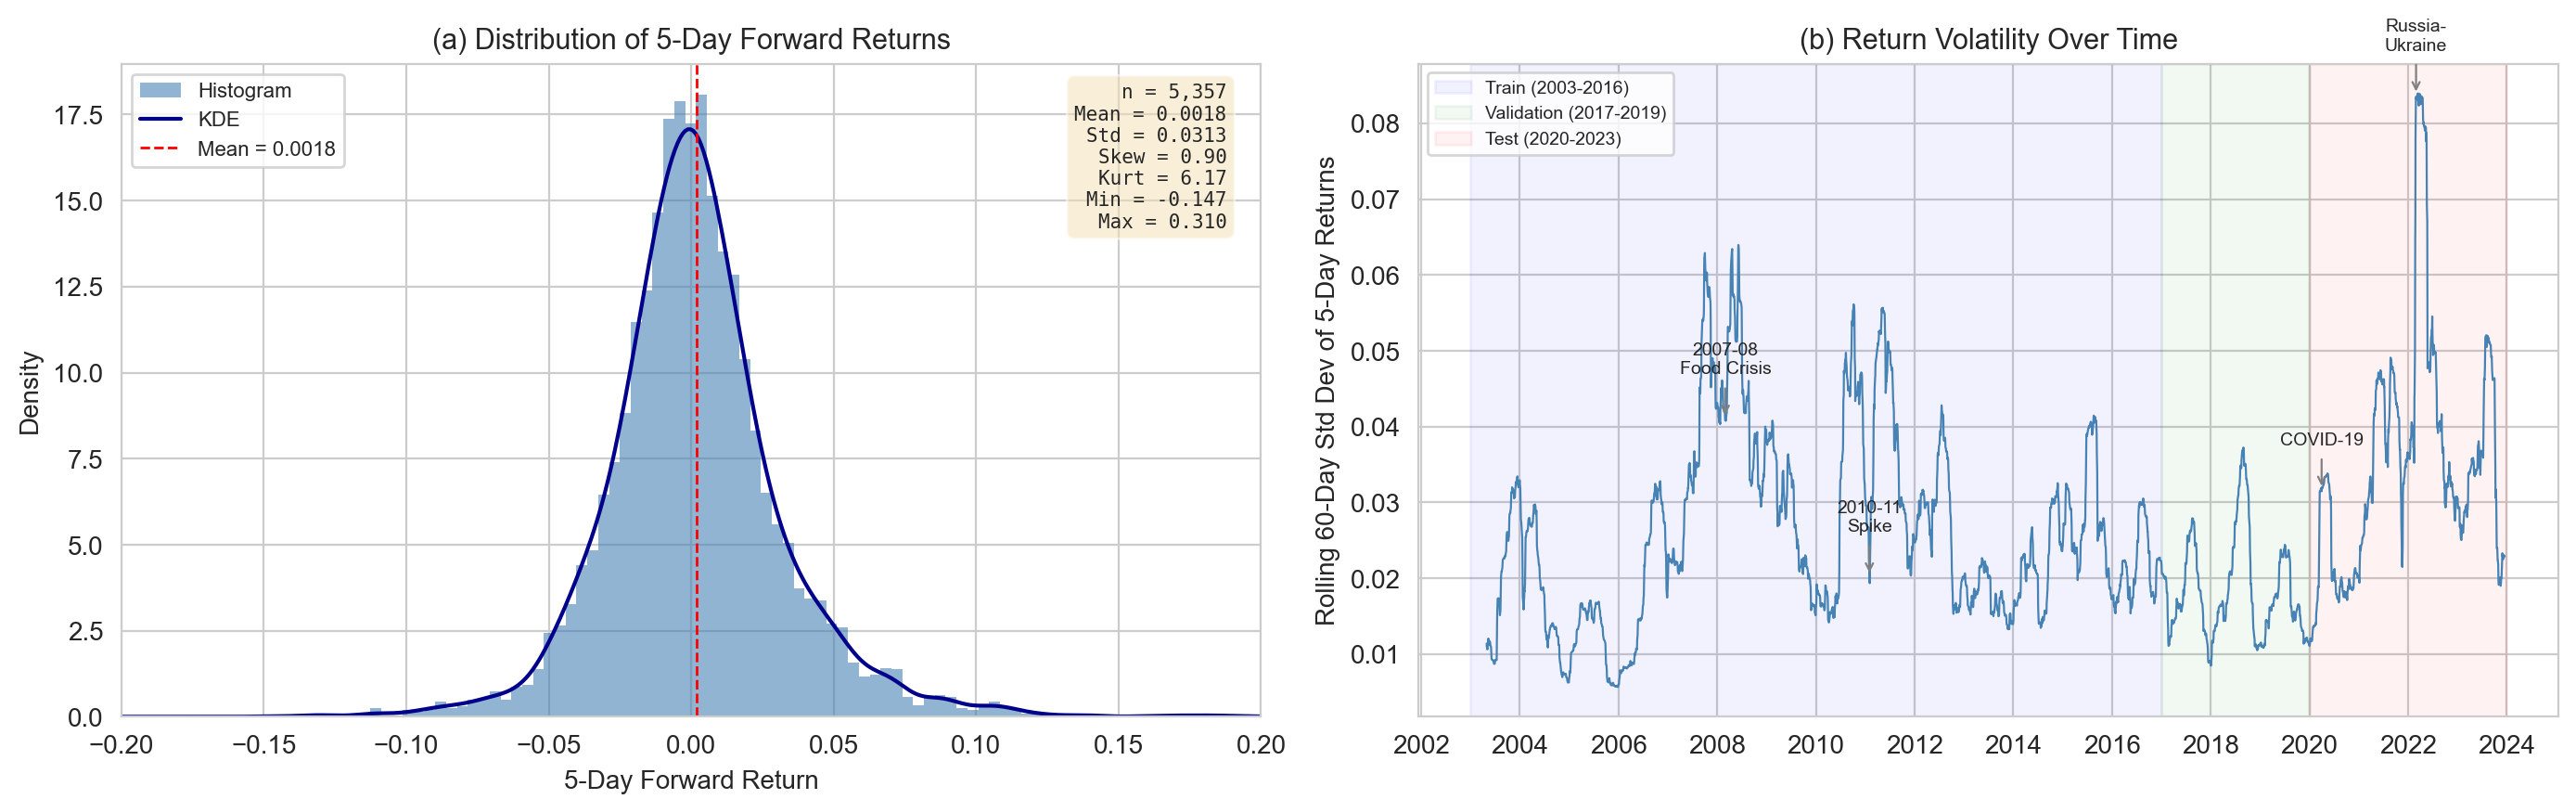
\includegraphics[width=\textwidth]{Figures/eda_return_distribution.png}
    \caption{(a) Distribution of 5-day forward returns for the Euronext Milling Wheat futures contract (2003-2023). The distribution is approximately symmetric with heavy tails (kurtosis = 6.17). (b) Rolling 60-day standard deviation of 5-day returns, with train/validation/test periods shaded. Volatility spikes correspond to the 2007-08 food crisis, COVID-19, and the 2022 Russia-Ukraine war.}
    \label{fig:return_dist}
\end{figure}

\subsection{Agricultural Feature Behaviour}

We now look at \autoref{fig:ag_vs_price} which plots the Euronext wheat futures 5-trading day returns alongside France-average NDVI and 30-day cumulative precipitation over the full sample period. We immediately see that returns are noisy and do not exhibit a trend while agricultural data is smooth and seasonal. Indeed, the agricultural variables exhibit strong annual seasonality: NDVI peaks each June-July when the wheat harvest areas reach maximum greenness, then declines after harvest, this repeats with high regularity across all twenty years. \autoref{fig:precipitation} in Appendix shows that cumulative precipitation fluctuates on a similar seasonal cycle but with much greater variability. In contrast, the futures return series shows no consistent seasonal pattern and can often be driven by geopolitical and macroeconomic events. Further, as mentioned in \autoref{sec:dataprep}, agricultural data is smooth on a daily timescale with NDVI updating every 8 days and fPAR every 10 days. This timescale mismatch is a key motivation for our choice of a 5-day (one-week) forecast horizon rather than a daily one: the slow-moving agricultural signals are unlikely to predict daily price variation, which is dominated by microstructure noise and order-flow dynamics~\cite{bib85} (See Section~\ref{sec:feature_eng} for more details). Additional EDA figures in  \autoref{app:eda} show that NDVI and fPAR are highly correlated ($\rho = 0.93$), however, they potentially diverge during cloudy periods (as NDVI is derived from satellite imagery), thus, we retain both in our feature set. Further, surface and root-zone soil moisture capture different timescales of water availability, thus, we keep both despite their near-perfect correlation of $\rho = 0.99$. Further, we see that the 2018 European drought produced 2.5 times the average number of hot stress days in Germany during the growing season, this drives our threshold-based stress features in Section~\ref{sec:feature_eng}.

\begin{figure}[H]
    \centering
    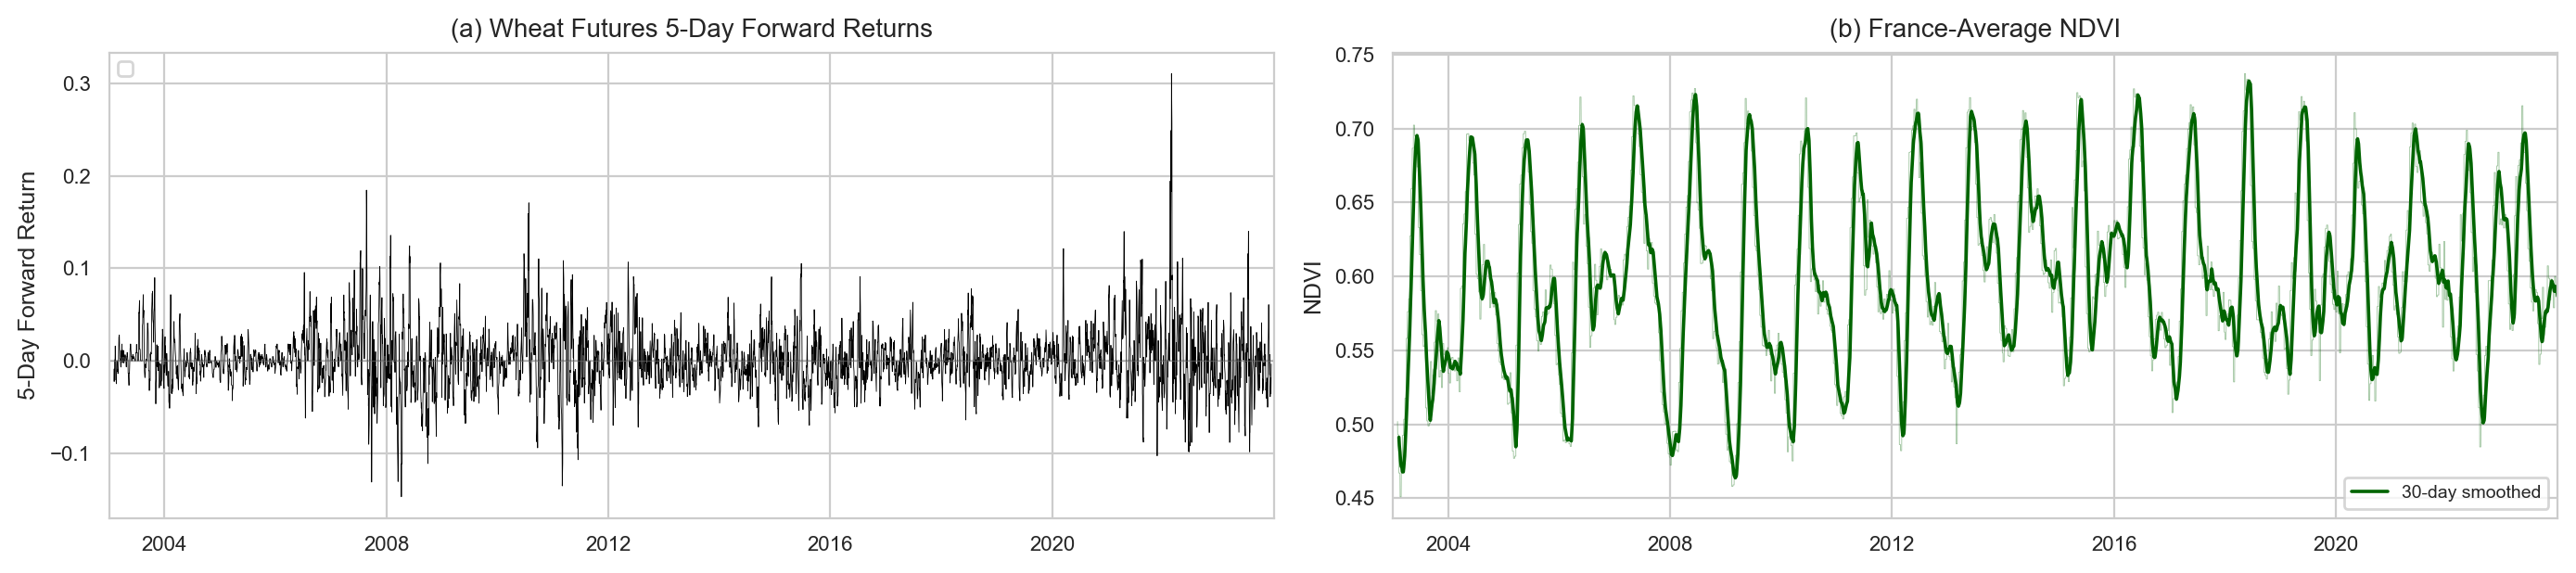
\includegraphics[width=\textwidth]{Figures/eda_ag_features_vs_price.png}
    \caption{(a) 5-day forward returns of the Euronext Milling Wheat futures, returns are noisy and display no seasonal pattern. (b) France-average NDVI with 30-day smoothing. NDVI 
    exhibits strong annual seasonality, peaking each June-July. The 
    timescale mismatch between the two series motivates the choice of a 
    weekly rather than daily forecast horizon.}
    \label{fig:ag_vs_price}
\end{figure}

\subsection{Feature Correlations}

\autoref{fig:corr_heatmap} in \autoref{app:eda} presents the Fisher z-averaged correlation matrix across all 507 regions for the 12 raw CY-Bench variables. Of the 66 unique feature pairs, 9 (13.6\%) exceed an absolute correlation of 0.85, with the highest being $|\rho| = 0.98$ between tmin and tavg. The most correlated group of features involves the temperature-related variables: tmin, tmax, tavg, et0, and vpd, which are all correlated above 0.80. This is expected since evapotranspiration and vapour pressure deficit are both derived from temperature inputs. As previously mentioned, surface and root-zone soil moisture are also highly correlated ($\rho = 0.97$). Precipitation stands out as largely uncorrelated with most other variables ($|\rho| < 0.33$), however, its correlation with the climatic water balance (cwb) is very high ($\rho = 0.94$) since cwb is computed as precipitation minus evapotranspiration. Although these patterns would introduce multicollinearity, we decide to keep all of these variables given that they represent distinct physical processes which may bring additional information to our models. We still verify the correlation of features during our feature engineering step in Section~\ref{sec:feature_eng}.

\subsection{Yield Distribution Across Countries}

Finally, we briefly examine the yield data for our secondary prediction task. \autoref{fig:yield_dist}(a) in \autoref{app:eda} shows that average wheat yields differ substantially across the three countries: Germany at 7.35 t/ha, France at 6.17 t/ha and Poland at 4.12 t/ha, reflecting differences in climate, soil quality, and farming intensity. Germany also exhibits the widest absolute spread across its 251 NUTS3 regions, with yields ranging from 2.57 to 11.04 t/ha. \autoref{fig:yield_dist}(b) plots the average yield trajectory over time. All three countries display a slight upward trend which could be driven by long-term improvements in crop varieties and management practices. Additionally, we see that, in 2018, all three countries experience a dip which corresponds to the European drought: Germany experienced a 7.3\% decline relative to other years, Poland 5.6\%, and France 2.9\%. These cross-country differences in yield level, variability, and drought sensitivity motivate our decision to tune model hyperparameters separately per country for the yield prediction task rather than using a single EU-wide configuration, as discussed in Section~\ref{sec:prediction_task}.

\section{Feature Engineering and Prediction Design}\label{sec:feature_eng}

Now that we have pre-processed and visualised our data, we add features and transform the data for model fitting for both prediction tasks. We start by describing the 14 engineered features for the futures prediction task, then we detail futures prediction target construction and temporal alignment, and finally we cover the yield forecasting pipeline.

\subsection{Engineered Features for the Futures Task}

Starting from the 12 raw daily CY-Bench variables per region, we create 14 additional features organised into five categories. These are driven by both patterns observed in the previous section as well as the agronomic literature.\\

Firstly, we follow CY-Bench's own feature design~\cite{bib17} by creating \textbf{threshold-based stress indicators}. We count cold days (tmin $< 0$\textdegree C), hot days (tmax $> 34$\textdegree C), and dry days (precipitation $< 1$\,mm) over rolling 30-day windows. We define hot days as $> 34$\textdegree C rather than $> 35$\textdegree C given that Tack et al.~\cite{bib_tack2015} show that above 34\textdegree C (in spring) wheat experiences the largest yield reduction. We further introduce ''grain-fill'' (which is when plants fill their grains from the nutrients they absorb) heat stress features for the May-July window using a 30\textdegree C threshold, counting both the number of exceedance days and the cumulative excess degrees above 30\textdegree C over 30-day windows. This lower threshold is motivated by Schlenker and Roberts~\cite{bib_schlenker2009}, who found that corn and soybean yield is negatively impacted beyond temperatures of 29 and 30\textdegree C, respectively. Although their study focuses on different crops, we lower the threshold to 30\textdegree C because, as per Porter and Gawith~\cite{bib_porter1999}, wheat is more sensitive to temperature during its  reproductive phase which includes grain-fill. Finally, we also compute spring heat shock indicators (tmax $> 25$\textdegree C during March-May) over 30-day and 60-day windows to capture early-season stress.\\

Secondly, fPAR enables us to compute \textbf{vegetation anomalies} relative to an expanding day-of-year climatology: $\text{anomaly}_{d,y} = \text{fPAR}_{d,y} - \bar{\text{fPAR}}_{d,<y}$, where $\bar{\text{fPAR}}_{d,<y}$ is the historical mean for that calendar day using only prior years. The expanding window avoids information leakage from future years. We retain both a raw daily anomaly and a 30-day rolling mean. This approach follows the near-real-time anomaly detection methodology of Meroni et~al.~\cite{bib_meroni2019}.\\

Thirdly, we compute a \textbf{drought feature} through a Standardised Precipitation Index (SPI)-like measure by z-scoring rolling 30-day and 60-day cumulative precipitation against its expanding historical distribution, following McKee et~al.~\cite{bib_mckee1993}. Positive values indicate wetter-than-normal conditions and negative values indicate drought.\\

Finally, a key additional feature to avoid information loss is a \textbf{weekend weather accumulator}. Indeed, since futures markets do not trade on weekends but weather events still occur, we accumulate 3-day precipitation (sum), maximum temperature, and minimum temperature on Mondays to capture the weekend weather surprise. This is motivated by the timescale mismatch observed in Section~\ref{sec:EDA}: agricultural data does not update over weekends while Monday returns must incorporate two days of unpriced information.\\

After our feature engineering, each region has 26 features (12 raw + 14 engineered). We intentionally exclude all price-derived features from our models since we want to focus on whether agricultural features from CY-Bench carry predictive power. Adding price features may lead our models to rely more on market data to make predictions as price derived features are directly impacted by different external factors and geopolitical events, which is not the case for agricultural data.

\subsection{Target Construction and Temporal Alignment}

As briefly mentioned in Section~\ref{sec:dataprep}, our target is not the raw daily return but the 5-trading-day forward return:
\begin{equation}
    y_{t} = \frac{P_{t+5}}{P_t} - 1
\end{equation}
where $P_t$ is the roll-adjusted closing price on day $t$. Since the ratio roll-adjustment preserves percentage returns across contract rolls, $y_t$ equals the compounded return a roll-following investor would experience over that window regardless of whether a roll occurred. We choose a 5-day horizon rather than a daily one because the EDA in Section~\ref{sec:EDA} showed that agricultural features evolve on weekly-to-monthly timescales while daily returns may be dominated by order-flow dynamics and other noise. Indeed, Deuskar and Johnson~\cite{bib85} found that flow-driven returns account for 40 to 70\% of market variance. This choice is also similar to Thaker et~al.~\cite{bib19}, who use a 20-trading-day horizon for their CNN-based wheat futures model. We include additional details on target construction in \autoref{app:target_construction}.\\

As a next step, to merge the regional agricultural features with the futures price data, we use a backward temporal join: for each trading day, each region is matched to its most recent agricultural observation on or before that date. Since both datasets are fully available for the February 2003 to December 2023 period defined in Section~\ref{sec:dataprep}, this merge introduces no missing values. All features are standardised to zero mean and unit variance before model fitting.\\

Since we have data for 507 regions, we choose to fit one model per region and then aggregate the predictions to EU-level. This aggregation follows Paudel et~al.~\cite{bib16}, who showed that regional models outperform nationally aggregated ones (in their yield task). This entails that once a separate model is fitted to each region, we aggregate the 507 per-region predictions into a single EU-level forecast by using production-weighted averaging:
\begin{equation}
    \hat{r}_{t+5}^{\text{EU}} = \frac{\sum_{r=1}^{R} w_{r,t}\, \hat{r}_{t+5}^{(r)}}{\sum_{r=1}^{R} w_{r,t}}
\end{equation}
where $w_{r,t} = \text{yield}_{r,t-1} \times \text{area}_{r,t-1}$ uses the previous year's production to avoid look-ahead bias. We note that for Germany, where CY-Bench provides harvest area only at census intervals, we forward-fill area within each region, which is the norm in operational European crop monitoring systems~\cite{bib_cerrani2017}. Finally, we note that by employing a one model per region scheme, we expose ourselves to the quality of the production data, which may introduce bias to our predictions given its annual frequency.

\subsection{Crop Yield Forecasting Pipeline}

While the primary contribution of this study is to test whether CY-Bench features predict futures returns, we also implement the task these features were designed for: sub-national wheat yield forecasting. This dual-task design serves as a positive control. If the agricultural features fail to predict both returns and yields, the negative futures result could reflect poor feature quality. If they predict yields well but not returns, the more interesting interpretation is that futures markets have already incorporated the agricultural information.\\

The yield pipeline aggregates daily CY-Bench time series into monthly summary features within each region's growing season, defined by the crop calendar start-of-season (SOS) and end-of-season (EOS) dates from CY-Bench. For each region-year pair, we compute monthly means for all meteorological, soil moisture, and vegetation variables over the available months, so that each observation is a single row with columns such as \texttt{ndvi\_mean\_oct}, \texttt{tmax\_mean\_mar}, etc. This preserves the temporal structure of the growing season while reducing dimensionality. Following CY-Bench's lead-time framework~\cite{bib17}, we build three separate datasets by truncating the available data at different points before harvest: end-of-season (all growing-season data available), mid-season (data truncated at $(SOS + EOS)/2$), and quarter-season (data truncated at $SOS + (EOS - SOS)/4$). These represent real-world forecasting scenarios where earlier predictions are more valuable but less accurate. We note that our monthly calendar-based aggregation differs from Paudel et~al.~\cite{bib16}, who aggregate by crop development phases using the WOFOST crop simulation model. Our approach is simpler and does not require crop model outputs, which CY-Bench does not provide.\\

The target variable is the official reported wheat yield in tonnes per hectare. We adopt a temporal split appropriate for the 2003--2020 data window: training on 2003--2014, validation on 2015--2017 (hyperparameter tuning only), and test on 2018--2020. The test period includes the 2018 European drought, providing a challenging evaluation. Following the cross-country differences in yield level and variability observed in Section~\ref{sec:EDA}, we tune hyperparameters separately for each country rather than using a single EU-wide configuration. We report normalised RMSE and $R^2$ at both per-region and production-weighted national levels, following CY-Bench~\cite{bib17}.

\section{Data Preparation}\label{sec:preprocessing}

This next section describes how we prepared two distinct datasets from the same underlying CY-Bench source: a daily-frequency panel for the wheat futures return prediction task (Section~\ref{subsec:futures_prep}), and an annual cross-section for the crop yield forecasting task (Section~\ref{subsec:yield_prep}). Although the data pre-processing of both tasks share the same raw CY-Bench sub-national dataset for France, Germany and Poland, they differ substantially in temporal granularity, target construction, and feature aggregation. We start by describing the futures prediction task pipeline first, as it constitutes the primary contribution of this study, and we also present the yield pipeline as our secondary task.

\subsection{Data Preparation for Wheat Futures Return Prediction}\label{subsec:futures_prep}

Firstly, our target variable data for the futures price prediction task is the Euronext Milling Wheat roll-adjusted daily closing prices obtained from Bloomberg for the period 01-01-2003 to 31-12-2023, yielding 5,389 trading days. More precisely, we define the raw target data as the closing price of the earliest maturing Euronext Milling Wheat Futures Contract given that near-term futures contracts are usually most liquid as per Ripple and Moosa ~\cite{bib84}. We use Bloomberg's ratio roll-adjustment to the time series 10 days before each contract expiry, this means that historical prices are multiplied by $P_{new \ contract} / P_{old \ contract}$ so as to preserve the percentage returns across all rolls. Our choice of $10$ days before expiry is arbitrary as, according to Carchano and Pardo's~\cite{bib25} study of stock index futures, choice of rollover timing does not induce statistically significant differences between the resulting return series. We note, however, that their study focuses on stock index futures rather than agricultural commodities which may exhibit stronger maturity effects due to seasonal supply factors. Further, as per L{\'o}pez de Prado Chapter~2 ~\cite{bib24}, our roll-adjustment eliminates the artificial jumps that occur at expiration to preserve the return dynamics experienced by a roll-following investor. This property is directly relevant to our study because the prediction target is a percentage return, not an absolute price level. A limitation of ratio adjustment is that it distorts historical price \emph{levels} (early-period prices may become very small or very large), making the series unsuitable for level-based analysis; however, since we use only returns and return-derived features, this limitation does not affect our study.

We retain two key fields from the raw data, closing price as well as volume. We note that Volume is forward-filled on dates where the field is reported as missing, a standard treatment for missing time series data to avoid data-leakage, in this case, this represents only 290 trading days or 5.4\% of trading days.

\subsubsection{Target variable: 5-day forward returns.}

After having extracted the raw target data from Bloomberg with the characteristics described above, we construct the prediction target as the 5 trading-day (one week) forward return:
\begin{equation}
    y_{t} = \frac{P_{t+5}}{P_t} - 1
\end{equation}
where  $P_{t}$ is the ratio-adjusted closing price on day $t$. Since the ratio adjustment maintains the percentage returns across rolls, $y_{t}$ equals the compounded return a roll-following investor would have experienced between days $t$ and $t+5$, regardless of whether a roll happened during that window. This is then framed as a regression problem so as to train the model to predict the continuous return rather than a binary (positive/negative) prediction task.

The reason for choosing 5-day horizon rather than 1-day stems from two key arguments. Firstly, on the predictor side, the agricultural features we use such as temperature, precipitation, NDVI and fPAR tend to evolve on weekly-to-monthly timescales. Thus, these slower moving variables may, by nature, be poor predictors of daily price movements. 

Secondly, in our dataset the NDVI and fPAR data is recorded weekly and three times a month respectively, meaning that we may not have data that is granular enough to be able to predict daily changes in futures price.  

A third key consideration is that, at a daily frequency, the price data may be dominated by market microstructure noise, order-flow dynamics, and intraday liquidity effects, for instance, Deuskar and Johnson ~\cite{bib85} found that flow-driven returns account for 40 to 70\% of market variance.

Finally, on the market side, the Samuelson hypothesis~\cite{bib54} predicts that futures price volatility increases as contracts approach expiration. Since we are looking at the closest maturing futures contract as our predictor, this implies that near-term price movements may display high variance which further justifies our 5-day time window choice. Indeed, Duong and Kalev~\cite{bib55} tested this hypothesis in 20 futures markets and found strong support specifically for agricultural commodities. On the other hand, while Daal et~al.~\cite{bib56} confirm that the Samuelson effect is more pronounced for commodities rather than financial futures, they find the effect to be absent from most contracts they test. Nevertheless, a weekly horizon enables us to reduce this higher-frequency noise while remaining a short enough time frame to be operationally relevant. This choice also mirrors Thaker et~al.~\cite{bib19}, who use a 20-trading-day forecast horizon for their CNN-based wheat futures prediction model, arguing that fundamentals-driven signals materialise over multi-day windows rather than at the daily frequency. We adopt the shorter 5-day window to retain more observations per test year while still filtering the majority of daily microstructure noise.

\subsubsection{Features - Argricultural data.}
Once we create our predictor vector, we look at CY-Bench to create our features. This dataset provides sub-national time series of meteorological variables (AgERA5: minimum and maximum temperature, precipitation, solar radiation, vapour pressure), soil moisture indicators (GLDAS), and satellite-derived vegetation indices (MODIS NDVI at 8-day resolution; JRC fPAR at dekadal resolution)~\cite{bib17}. We load data for 515 regions across France (97 NUTS3), Germany (397 NUTS3), and Poland (17 NUTS2), which collectively account for the three largest wheat-producing countries in the European Union.

Each data type arrives at its native temporal resolution: daily for weather and soil moisture, 8-day for NDVI, and dekadal (approximately 10-day) for fPAR. Following CY-Bench's own pre-processing protocol (\cite{bib17}, Section~2.2.2), we retain these heterogeneous frequencies and expand them to daily granularity per region using last-observation-carried-forward (LOCF) interpolation, which fills each day with the most recently observed value. LOCF is a standard approach for remote sensing time series that avoids introducing information from future observations~\cite{bib_meroni2019} and is the default method used in operational agricultural monitoring systems such as the JRC MARS Crop Yield Forecasting System~\cite{bib_cerrani2017}. After expansion, each region's daily DataFrame contains a consistent set of raw variables aligned to a common daily calendar.

\subsubsection{Temporal alignment between agricultural and price data.}
A central challenge is that the agricultural data are available at regional (sub-national) level on a daily or sub-daily calendar, while futures prices exist only on trading days and represent a single EU-wide market. We merge these two frequencies using an \emph{asof} (backward) temporal join: for each trading day, each region is matched to its most recent available agricultural observation on or before that date. This ensures strict temporal causality-no future agricultural information is used to predict current returns. This backward-join approach is standard in event-study and cross-asset prediction literature, where low-frequency fundamental data must be aligned with higher-frequency price data without lookahead bias~\cite{bib_kapoor2023}. After the merge, any remaining missing values in agricultural columns are forward-filled and then zero-filled as a final fallback, ensuring that the feature matrix contains no NaN entries.

\subsubsection{Production weights and look-ahead avoidance.}
To aggregate per-region predictions to the EU level (see Section~\ref{sec:prediction_task}), we compute production weights as $w_{r,t} = \text{yield}_{r,t-1} \times \text{area}_{r,t-1}$, using the \emph{previous} year's production to avoid look-ahead bias. This follows the approach of Paudel et~al.~\cite{bib16}, who aggregate regional predictions to national level using crop area weights and demonstrate that this bottom-up aggregation produces forecasts competitive with nationally-calibrated systems.

A practical complication arises for Germany, where CY-Bench provides harvest area data only at census intervals (approximately every four years), with the \texttt{production} column entirely missing. We address this by forward-filling harvest area within each region across years and computing production as yield $\times$ forward-filled area. This is standard practice in European agricultural statistics: Eurostat publishes area data at lower frequency than yield, and Cerrani and L\'opez Lozano~\cite{bib_cerrani2017} document that carry-forward interpolation of area data is the norm in operational crop monitoring systems such as MCYFS. French and Polish data have complete annual area and production columns and require no imputation.

\subsubsection{Feature engineering.}
Starting from the raw daily variables, we engineer 76 features per region organised into five categories, each motivated by agronomic or climate science literature:

\paragraph{Rolling aggregates.} We compute 30-day and 60-day rolling means and cumulative sums for core weather variables. These windows capture medium-term climate trends that are known to drive crop development outcomes~\cite{bib16}.

\paragraph{Threshold-based stress indicators.} Following CY-Bench's feature design (\cite{bib17}, Section~2.2.3), we count cold days (minimum temperature $< 0 \degree$C), hot days (maximum temperature $> 35\degree$C), and dry days (precipitation $< 1$\,mm) over 30-day windows. We further introduce grain-fill heat stress indicators (days with maximum temperature $> 30\degree$C during May-July), motivated by Schlenker and Roberts~\cite{bib_schlenker2009}, who demonstrate a sharply nonlinear relationship between temperature above crop-specific thresholds and US crop yields, with damages accelerating beyond approximately 29-32\degree C.

\paragraph{Vegetation anomalies.} For fPAR, we compute anomalies relative to an expanding day-of-year climatology: $\text{anomaly}_{d,y} = \text{fPAR}_{d,y} - \bar{\text{fPAR}}_{d,<y}$, where $\bar{\text{fPAR}}_{d,<y}$ is the historical mean for that calendar day using only data from prior years. The expanding (rather than fixed) climatology avoids information leakage from future years. This anomaly approach is standard in operational vegetation monitoring; Meroni et~al.~\cite{bib_meroni2019} adopt a similar methodology for near-real-time NDVI anomaly detection within the JRC's food security monitoring framework.

\paragraph{Drought index.} We compute a Standardised Precipitation Index (SPI)-like measure by z-scoring rolling 30-day and 60-day cumulative precipitation against its expanding historical distribution. This follows the methodology of McKee et~al.~\cite{bib_mckee1993}, who introduced the SPI as a standardised drought severity metric, now widely used in agricultural drought monitoring worldwide.

\paragraph{Weekend weather accumulator.} Since futures markets do not trade on weekends but weather events still occur, we accumulate 3-day precipitation, maximum temperature, and minimum temperature on Mondays to capture the weekend weather surprise that the market prices on the first trading day of the week.
%% FLAG: This feature lacks a direct academic citation. While the logic is sound from a market microstructure perspective (markets react to accumulated news upon reopening), we could not find a published paper that specifically validates this weekend-weather-accumulator feature for commodity futures. You may wish to either (a) provide an empirical justification from your EDA, (b) cite a general market microstructure reference on information incorporation after market closures, or (c) remove this feature if reviewers challenge it.

\subsubsection{Correlation-based feature filtering.}
Before modelling, we compute an average cross-regional correlation matrix using Fisher's z-transformation~\cite{bib_fisher1921}: each region's pairwise feature correlation matrix is transformed via $z = \text{arctanh}(r)$, averaged across all 515 regions in the z-domain, and back-transformed via $r = \text{tanh}(\bar{z})$. Feature pairs with average absolute correlation exceeding 0.85 are flagged, and one feature from each highly correlated pair is dropped. This avoids multicollinearity, which inflates the variance of coefficient estimates in regularised linear models~\cite{bib_hastie2009}. The Fisher z-averaging is necessary because raw correlations are bounded and skewed, making arithmetic averaging of correlations across regions statistically inappropriate~\cite{bib_fisher1921}.

\subsubsection{Minimal price features.}
A critical design choice is to restrict price-derived features to only three variables: 5-day return, 20-day return, and a volume-to-moving-average ratio. This minimal set provides the model with basic information about recent price momentum and market attention, but deliberately excludes technical indicators (RSI, Bollinger bands, moving average crossovers) commonly used in price forecasting. The rationale is that our research question asks whether \emph{agricultural} features from CY-Bench add predictive power for futures returns. Including a rich set of price-based features would confound the agricultural signal with price feature interactions, making it impossible to attribute any predictive lift to the CY-Bench data. This controlled ablation design is consistent with the ICML best practices recommendation that experiments should be designed to answer specific research questions~\cite{bib_goodfellow2016}.


\subsection{Data Preparation for Crop Yield Forecasting}\label{subsec:yield_prep}

The yield forecasting task uses the same CY-Bench source data but requires a fundamentally different preparation pipeline, as the target is annual end-of-season yield (tonnes per hectare) rather than daily futures returns.

\subsubsection{Temporal scope and region filtering.}
We restrict the yield analysis to harvest years 2003-2020 and retain only the 357 regions (90 French, 251 German, 16 Polish) that report yield statistics for every year in this 18-year window. The start year is determined by the availability of GLDAS soil moisture data, which begins in February 2003~\cite{bib17}. The end year is constrained by the latest available sub-national yield statistics: the JRC harmonised European dataset~\cite{bib_ronchetti2024} provides French NUTS3 yields through 2020, German NUTS3 yields through 2021, and Polish NUTS2 yields through 2020. We adopt the binding constraint of 2020 to maintain a balanced panel.

This filtering is conservative in information loss: the 357 retained regions account for 97.5\% of total wheat production across the three countries (99.9\% for France, 93.3\% for Germany, 99.4\% for Poland), confirming that the dropped regions are predominantly small districts with discontinued reporting rather than major wheat-producing areas. Ensuring complete temporal coverage for every retained region is a prerequisite for fair cross-regional comparison under the walk-forward evaluation scheme.

\subsubsection{Monthly feature aggregation with lead-time truncation.}
Unlike the futures pipeline, which uses daily features, the yield pipeline aggregates daily CY-Bench time series into monthly summaries within each region's growing season. For each region-year pair, we extract the growing season window (defined by the crop calendar's start-of-season and end-of-season dates from CY-Bench) and compute monthly means, sums, and extremes for all meteorological, soil moisture, and vegetation variables. This monthly aggregation reduces the dimensionality from thousands of daily observations to tens of features while preserving the temporal structure of the growing season.

Following CY-Bench's lead-time framework (\cite{bib17}, Section~3.2), we build three separate datasets by truncating the available data at different points before harvest: \emph{end-of-season} (all growing-season data available), \emph{mid-season} (data truncated at $(SOS + EOS)/2$), and \emph{quarter-season} (data truncated at $SOS + (EOS - SOS)/4$). These correspond to real-world forecasting scenarios with decreasing information but increasing decision-making value. Each region-year pair becomes a single observation, with the target being the official reported yield in tonnes per hectare.

We note that our monthly aggregation differs from the methodology of Paudel et~al.~\cite{bib16}, who aggregate daily data by crop development phases identified through the WOFOST crop simulation model (e.g., emergence, flowering, grain-fill). Our approach is simpler and does not require crop model outputs, which CY-Bench does not provide~(\cite{bib17}, Section~4.2, Limitation~3). This trade-off means we sacrifice some agronomic precision for broader applicability and reproducibility.

\section{Prediction Tasks}\label{sec:prediction_task}

This section defines the two prediction tasks addressed in this study. We first describe the primary task-predicting wheat futures returns from agricultural features-and then present the secondary task of crop yield forecasting, which serves both as a validation of the agricultural features' information content and as a benchmark against established results.

\subsection{Primary Task: Wheat Futures Return Prediction}\label{subsec:futures_task}

\subsubsection{Target variable: 5-day forward returns.}
We define the prediction target as the 5-trading-day (one week) forward log return of the Euronext Milling Wheat N2 futures contract:
\begin{equation}
    r_{t+5} = \frac{P_{t+5}}{P_t} - 1
\end{equation}
where $P_t$ is the roll-adjusted closing price on day $t$. We frame this as a regression problem, predicting the continuous return rather than the binary direction.

The choice of a 5-day horizon, rather than 1-day, is motivated by both the structure of our data and the nature of the prediction problem. Agricultural features such as growing-season temperature and NDVI evolve on weekly-to-monthly timescales, making it implausible that they would predict \emph{daily} price variation, which is dominated by microstructure noise, order-flow dynamics, and intraday liquidity effects. A weekly horizon filters out much of this high-frequency noise while remaining short enough to be operationally relevant. This choice mirrors Thaker et~al.~\cite{bib19}, who use a 20-trading-day forecast horizon for their CNN-based wheat futures prediction model, arguing that fundamentals-driven signals materialise over multi-day windows rather than at the daily frequency. More broadly, the efficient market hypothesis~\cite{bib_fama1970} implies that publicly available information is rapidly incorporated into prices; any residual agricultural signal is more likely to manifest at lower frequencies where markets have not yet fully digested supply-side information.

\subsubsection{Per-region models with production-weighted aggregation.}
With 515 regions and 76 agricultural features per region, directly concatenating all features into a single vector would produce 39,140 input dimensions-far exceeding the approximately 5,000 available observations. Goodfellow et~al.~\cite{bib_goodfellow2016} warn that this regime requires strong regularisation. We address this by fitting one model per region using only that region's features plus the three price features (79 features total), and then aggregating the 515 per-region predictions into a single EU-level forecast using production weights.

This per-region approach is motivated by Paudel et~al.~\cite{bib16}, who demonstrated that building models at the regional level and aggregating to larger spatial units produces lower normalised RMSE than building a single model on nationally aggregated predictors. They attribute this to reduced aggregation error: predictors at regional level correlate better with local outcomes because spatial averaging masks regional heterogeneity. Chipanshi et~al.~\cite{bib_chipanshi2015} corroborate this finding using Canadian data, showing that predicting yields at smaller spatial units and aggregating upward produces better results than aggregating predictors first.

For the aggregation step, we use the production-weighted average:
\begin{equation}
    \hat{r}_{t+5}^{\text{EU}} = \frac{\sum_{r=1}^{R} w_{r,t}\, \hat{r}_{t+5}^{(r)}}{\sum_{r=1}^{R} w_{r,t}}
\end{equation}
where $\hat{r}_{t+5}^{(r)}$ is region $r$'s predicted return and $w_{r,t}$ is the prior-year production weight. Regions with larger wheat output thus contribute more to the aggregate prediction, reflecting the intuition that supply shocks in major producing regions have greater price impact than those in minor ones.

\subsubsection{Walk-forward evaluation with temporal partitioning.}
We adopt a strictly chronological train/validation/test split:
\begin{itemize}
    \item \textbf{Training}: 2003-2016 (14 years, $\sim$3,600 trading days);
    \item \textbf{Validation}: 2017-2019 (3 years, used exclusively for hyperparameter tuning);
    \item \textbf{Test}: 2020-2023 (4 years, never seen during model selection).
\end{itemize}
Random train-test splits are inappropriate for time series data because they create temporal leakage-the model trains on data that chronologically follows the test set, inflating performance estimates. Kapoor and Narayanan~\cite{bib_kapoor2023} document that such leakage is a leading cause of irreproducibility in ML-based science, affecting a substantial fraction of published results. Paudel et~al.~\cite{bib16} adopt an analogous time-based look-forward cross-validation for crop yield prediction, training only on years preceding each test year. Our three-way split further isolates hyperparameter tuning from final evaluation, following the standard ML workflow described in Goodfellow et~al.~\cite{bib_goodfellow2016}.

The training set is designed to include both the 2007-2008 global food price crisis (wheat prices rose by 136\%) and the 2010-2011 secondary spike, ensuring the model sees volatile periods. The test period (2020-2023) provides a challenging out-of-sample evaluation encompassing COVID-19 supply chain disruptions and the 2022 Russia-Ukraine war, during which wheat prices surged to their highest levels since 2008. This design follows the ICML best practice of selecting test conditions that stress the model's generalization.

\subsubsection{Hyperparameter tuning.}
We use randomised search over 20 parameter combinations per model, following Bergstra and Bengio~\cite{bib_bergstra2012}, who prove that random search is more efficient than grid search for hyperparameter optimization when some hyperparameters are more important than others-a condition that holds for most ML models. Tuning is performed on the validation set only; the test set is never used for model selection.

\subsubsection{Models evaluated.}
We test four model families: Ridge Regression, Lasso Regression, Random Forest, and Extremely Randomised Trees (ExtraTrees). These represent increasing levels of nonlinearity while remaining interpretable. Ridge and Lasso are regularised linear models that differ in their penalty structure ($L_2$ versus $L_1$), with Lasso additionally performing implicit feature selection through coefficient shrinkage to zero~\cite{bib_hastie2009}. Random Forest and ExtraTrees are ensemble methods based on decision trees that can capture nonlinear interactions between features without manual feature crossing. All features are standardised (zero mean, unit variance) before fitting, which is necessary for the regularisation penalties in Ridge and Lasso to weight all features equally~\cite{bib_hastie2009}. A deep neural network component is planned but not yet implemented.
%% FLAG: The neural network section is currently empty in the notebook (Cell 35 contains only a comment). This should either be implemented before submission or explicitly removed from the methods description.


\subsection{Secondary Task: Crop Yield Forecasting}\label{subsec:yield_task}

\subsubsection{Motivation for a dual-task design.}
While the primary contribution of this study is to test whether CY-Bench features predict futures returns, the yield forecasting task serves two complementary purposes. First, it provides a \textbf{positive control}: if the same agricultural features that fail to predict futures returns also fail to predict crop yields, the negative futures result could be attributed to poor feature quality rather than market efficiency. If, however, the features predict yields well but not returns, the result supports the interpretation that futures markets efficiently incorporate agricultural information. Second, the yield task allows \textbf{direct comparison with established benchmarks}. Paudel et~al.~\cite{bib16} and the CY-Bench benchmark~\cite{bib17} provide published results for exactly this task, enabling us to verify that our data preparation pipeline is correct and that our model implementations are competitive.

\subsubsection{Target and lead times.}
The target variable is end-of-season wheat yield in tonnes per hectare, as reported in official sub-national statistics. Following the CY-Bench protocol~\cite{bib17}, we evaluate at three lead times-end-of-season, mid-season, and quarter-season-to assess how forecast accuracy degrades when less growing-season information is available. This lead-time structure mirrors real-world operational forecasting, where earlier predictions are more valuable but less accurate~\cite{bib16}.

\subsubsection{Walk-forward evaluation.}
We adopt a temporal split appropriate for the 2003-2020 data window:
\begin{itemize}
    \item \textbf{Training}: 2003-2014 (12 years $\times$ 357 regions $\approx$ 4,300 observations);
    \item \textbf{Validation}: 2015-2017 (hyperparameter tuning only);
    \item \textbf{Test}: 2018-2020.
\end{itemize}
This is the same walk-forward design described above, but with boundaries shifted to fit the shorter available time span. The test period includes the 2018 European drought-one of the most severe on record for wheat, with German yields dropping sharply-making this a challenging evaluation. As Paudel et~al.~\cite{bib16} note, the practical value of yield forecasting models depends critically on their performance during extreme years, which is when stakeholders most need accurate predictions.

\subsubsection{Per-country tuning.}
For the yield task, we tune hyperparameters separately for each country rather than using a single EU-wide configuration. This reflects the fact that the relationship between growing-season climate and yield varies across agro-climatic zones; French Atlantic maritime wheat systems respond differently to the same temperature anomaly than German continental systems. Per-country tuning allows the model to adapt its regularisation strength and tree depth to the local signal-to-noise ratio.

\subsubsection{Metrics.}
Following CY-Bench~\cite{bib17}, we report normalised root mean squared error (NRMSE = RMSE divided by mean observed yield) and $R^2$ at both the per-region and production-weighted national levels. NRMSE facilitates cross-country comparison because it is scale-invariant, while $R^2$ quantifies the proportion of yield variance explained.

\clearpage

\section{Method 1 (2 pages)}\label{ridge_lasso}

\clearpage

\section{Method 2 (2 pages)}\label{rf_et}

\clearpage

\section{Method 3 (2 pages)}\label{neuralnets}

\clearpage

\section{Model Result Comparison (1 page)}\label{result_comparison}

\clearpage

\section{Conclusion (1 page)}\label{conclusion}

\clearpage

\bibliography{sn-bibliography}% common bib file
%% if required, the content of .bbl file can be included here once bbl is generated
%%\input sn-article.bbl

\clearpage

\section{Generative AI Statement}

\clearpage

\begin{appendices}

\section{Excluded Regions for the Wheat Futures Prediction Task}\label{A1}

% Excluded French NUTS3 regions (total= 101, our total=94): FR101 Paris, FR105 Hauts-de-Seine, FRY10 Guadeloupe, FRY20 Martinique, FRY30 French Guiana, FRY40 La Reunion, FRY50 Mayotte -> resulting in a total of 94 regions
% Excluded German NUTS3 regions(total= 400, our total=397): DE300 Berlin, DE501 Bermen Kreisfreie Stadt, DE502 Bremerhaven Kreisfreie Stadt, DE600 Hamburg -> resulting in a total of 397 regions

\begin{table}[htbp]
\centering
\caption{Classification of Select NUTS Regions by Primary Geographic and Economic Function}
\label{tab:region_classification}
\begin{tabular}{llll}
\toprule
\textbf{Category} & \textbf{NUTS Code} & \textbf{Region Name} & \textbf{Rationale \& Source} \\
\midrule
\textbf{Urban Center} 
& FR101 & Paris & Capital city, dense urban core \cite{insee_stats} \\
& FR105 & Hauts-de-Seine & High-density inner Parisian suburb \cite{insee_stats} \\
& DE300 & Berlin & German capital and city-state \cite{destatis_stats} \\
\midrule
\textbf{Logistic Hub} 
& DE600 & Hamburg & 3rd largest port in Europe \cite{hamburg_port} \\
& DE501 & Bremen & Major maritime/freight center \cite{destatis_stats} \\
& DE502 & Bremerhaven & Key international seaport \cite{bremenports_stats} \\
& DE945 & Wilhelmshaven & Coastal industrial hub \cite{jadeweserport_stats} \\
\midrule
\textbf{Non-wheat Producing} 
& FRY10 & Guadeloupe & Tropical climate; sugarcane/bananas \cite{agreste_stats} \\
\textbf{(Tropical / Overseas)} 
& FRY20 & Martinique & Tropical climate; sugarcane/bananas \cite{agreste_stats} \\
& FRY30 & French Guiana & Equatorial rainforest climate \cite{agreste_stats} \\
& FRY40 & La Réunion & Tropical island climate \cite{agreste_stats} \\
& FRY50 & Mayotte & Tropical island climate \cite{agreste_stats} \\
\bottomrule
\end{tabular}
\end{table}

\section{Supplementary EDA Figures}\label{app:eda}

\begin{figure}[ht]
    \centering
    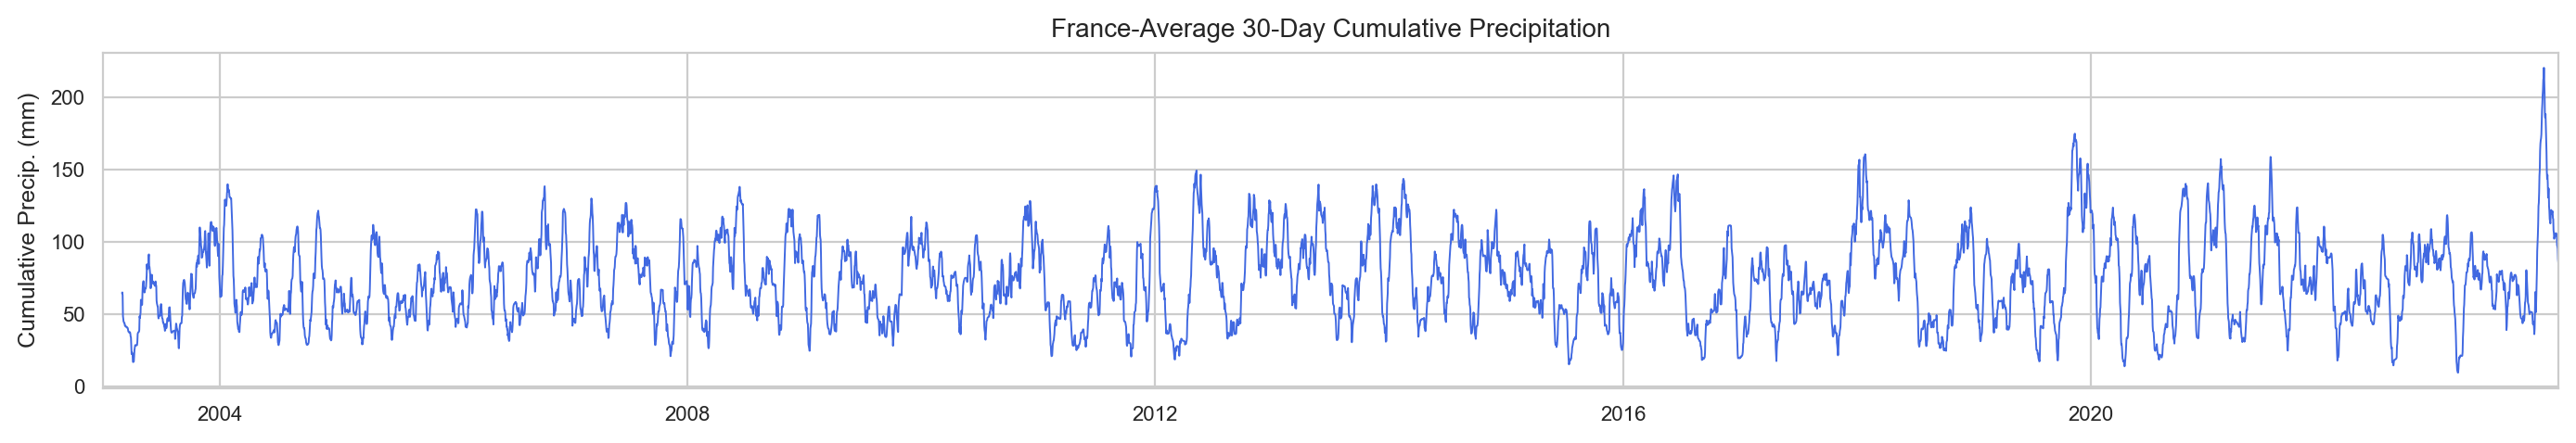
\includegraphics[width=\textwidth]{Figures/eda_precipitation.png}
    \caption{France-average 30-day cumulative precipitation (2003-2023). Precipitation fluctuates on a seasonal cycle with substantial inter-annual variability but, unlike NDVI, lacks a consistent repeating pattern, reflecting the stochastic nature of rainfall events.}
    \label{fig:precipitation}
\end{figure}

\begin{figure}[ht]
    \centering
    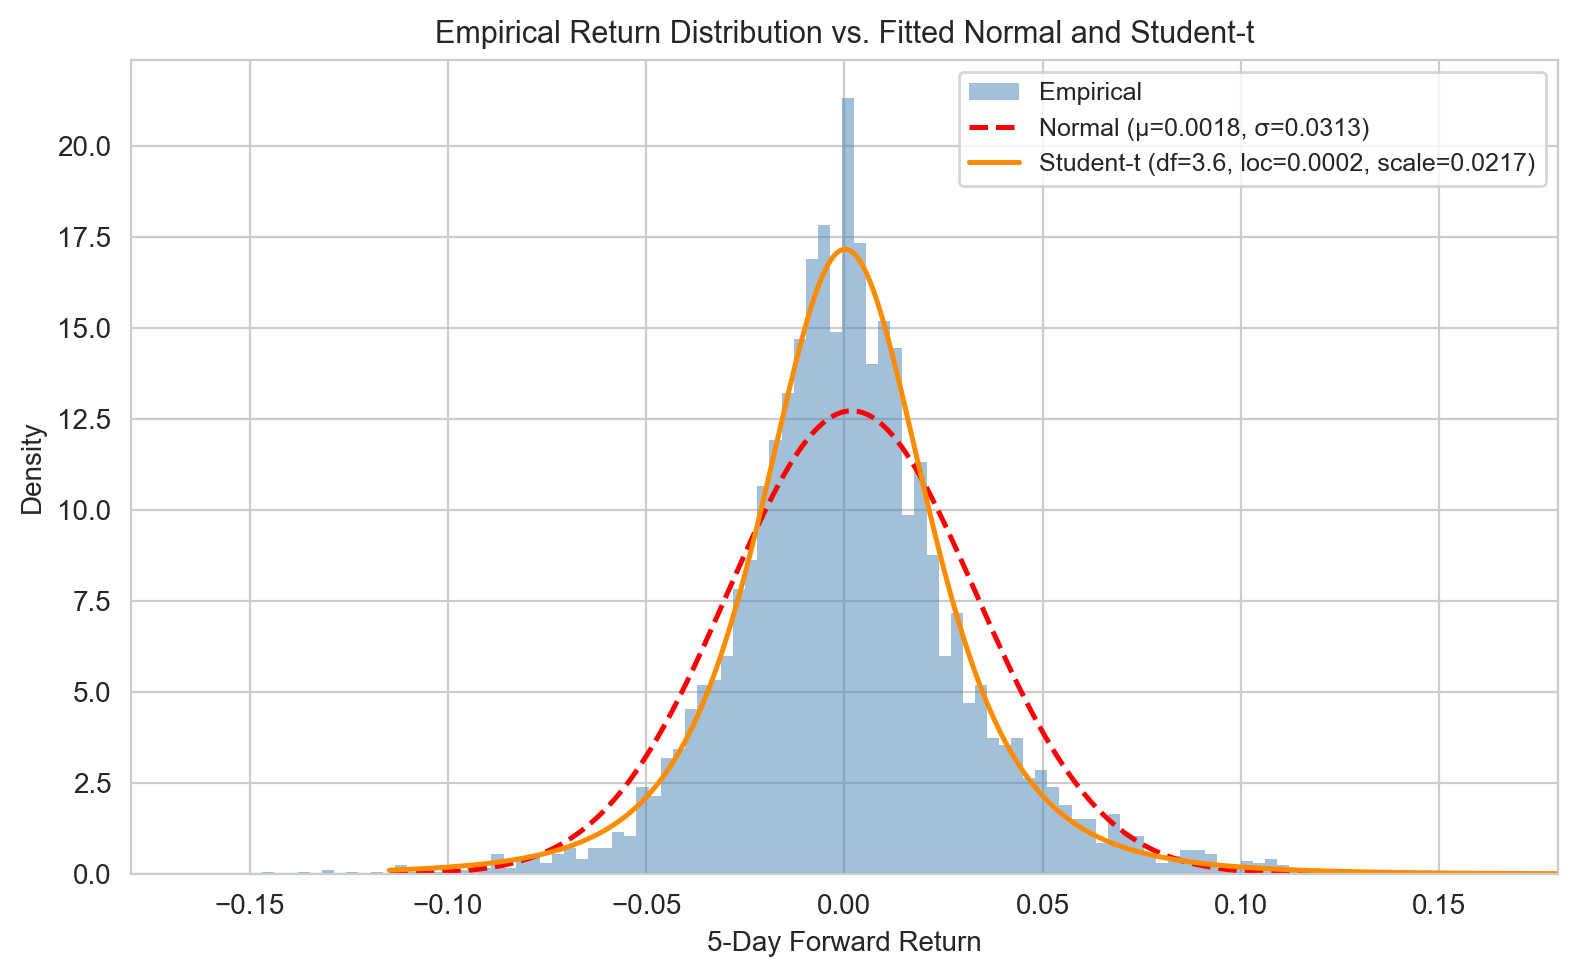
\includegraphics[width=0.75\textwidth]{Figures/eda_return_vs_theoretical.png}
    \caption{Empirical 5-day return distribution compared with fitted Normal and Student-t densities. The fitted Student-t has 3.6 degrees of freedom, confirming substantially heavier tails than the Gaussian benchmark.}
    \label{fig:return_vs_t}
\end{figure}

\begin{figure}[ht]
    \centering
    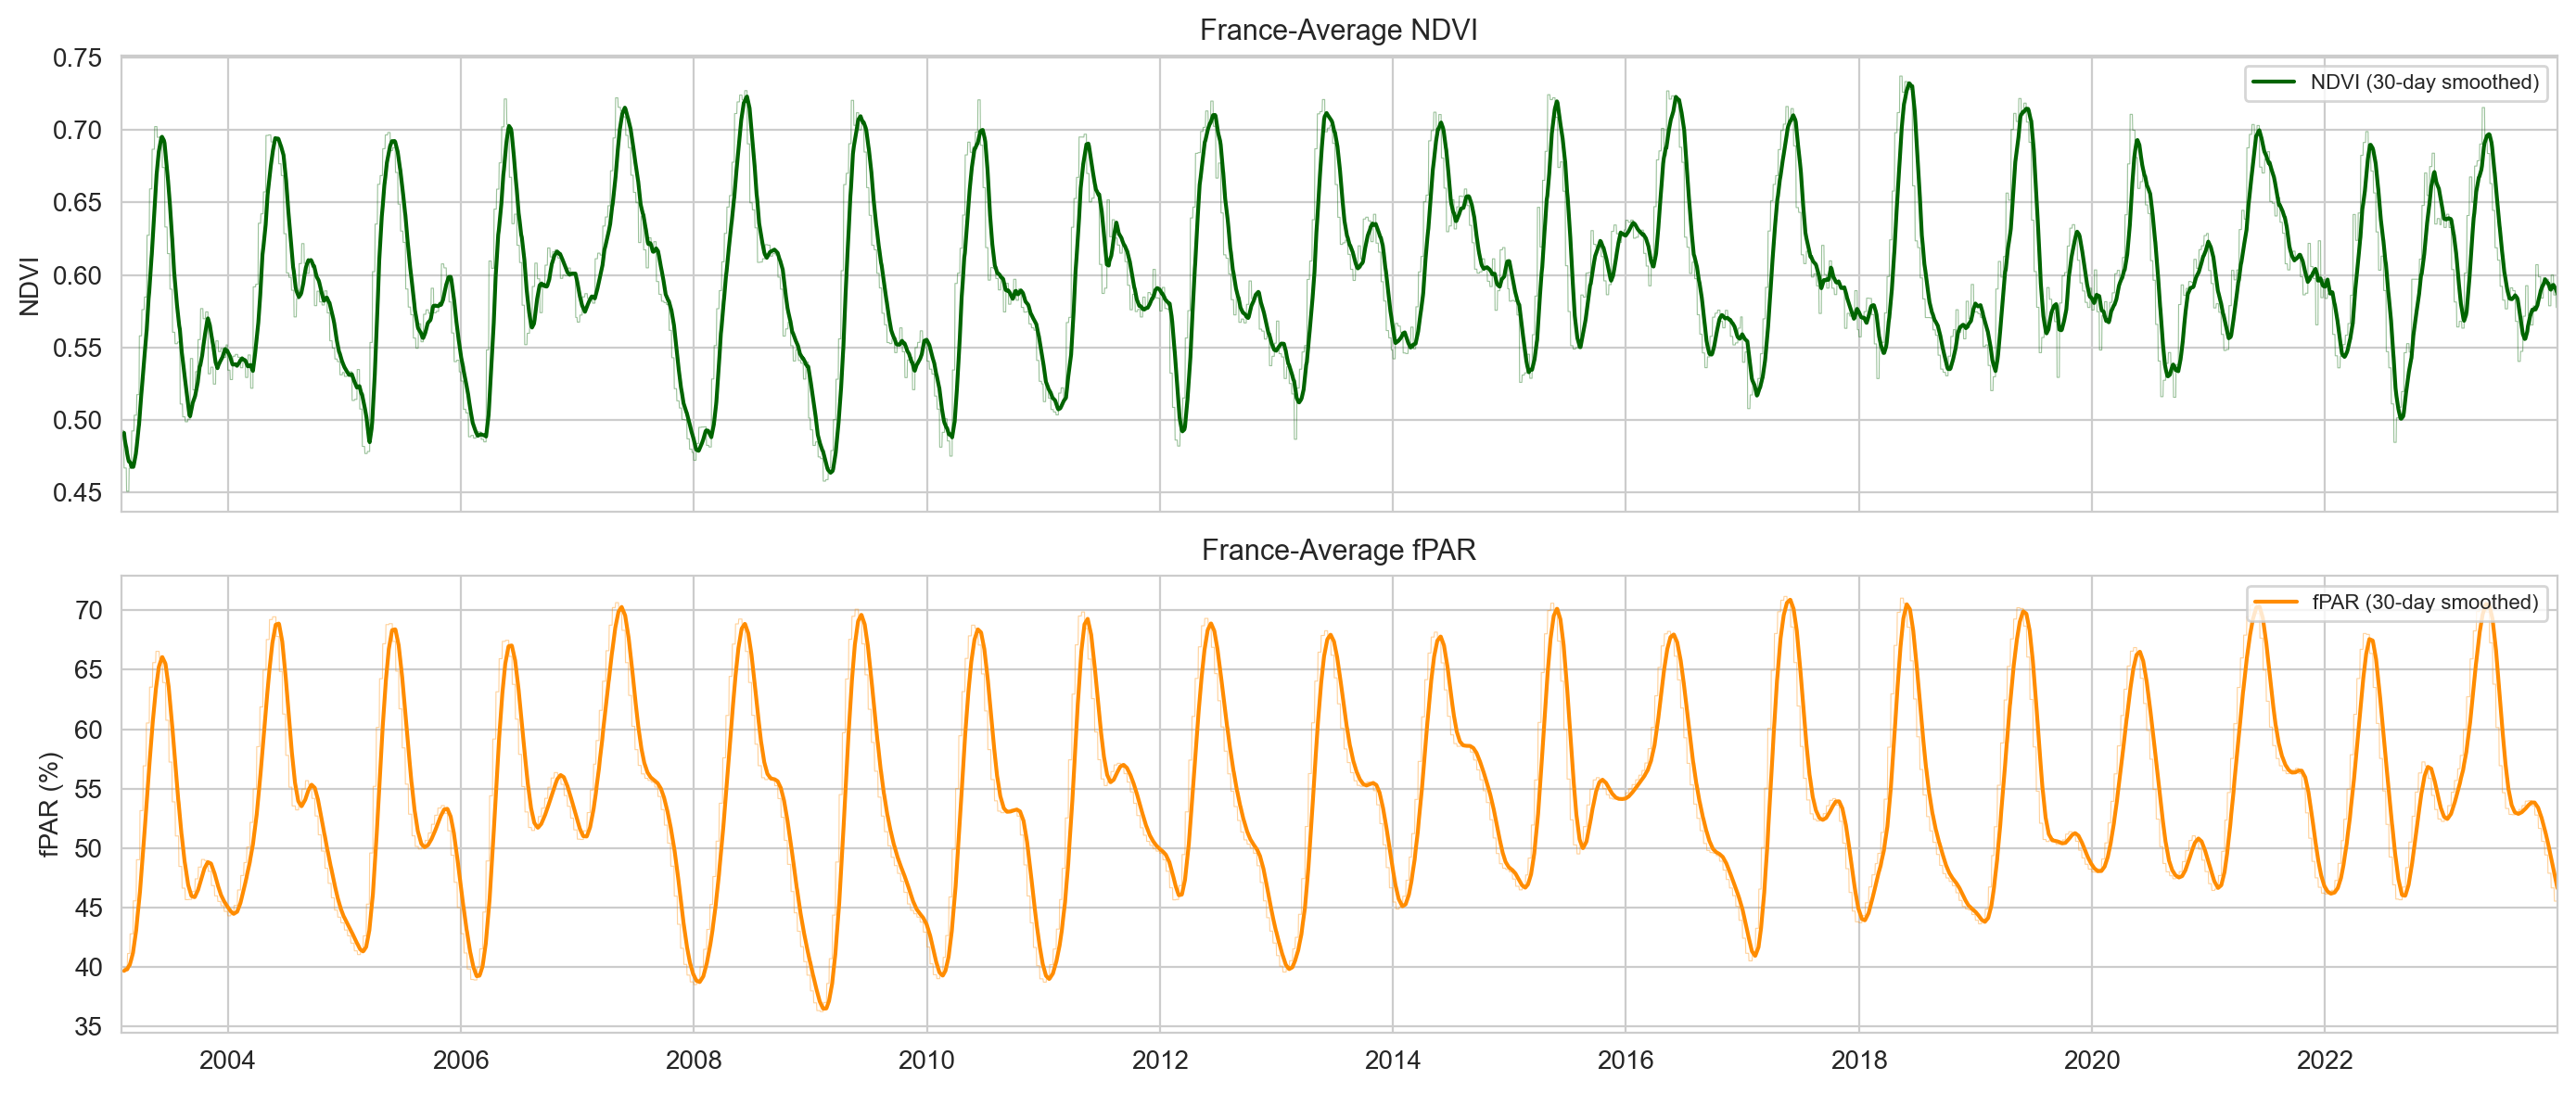
\includegraphics[width=\textwidth]{Figures/eda_ndvi_vs_fpar.png}
    \caption{France-average NDVI (top) and fPAR (bottom), 2003-2023. Both indicators track each other closely ($r = 0.93$ on 30-day smoothed series) but diverge during cloud-contaminated periods due to different gap-filling methods, justifying retaining both in the feature set.}
    \label{fig:ndvi_fpar}
\end{figure}

\begin{figure}[ht]
    \centering
    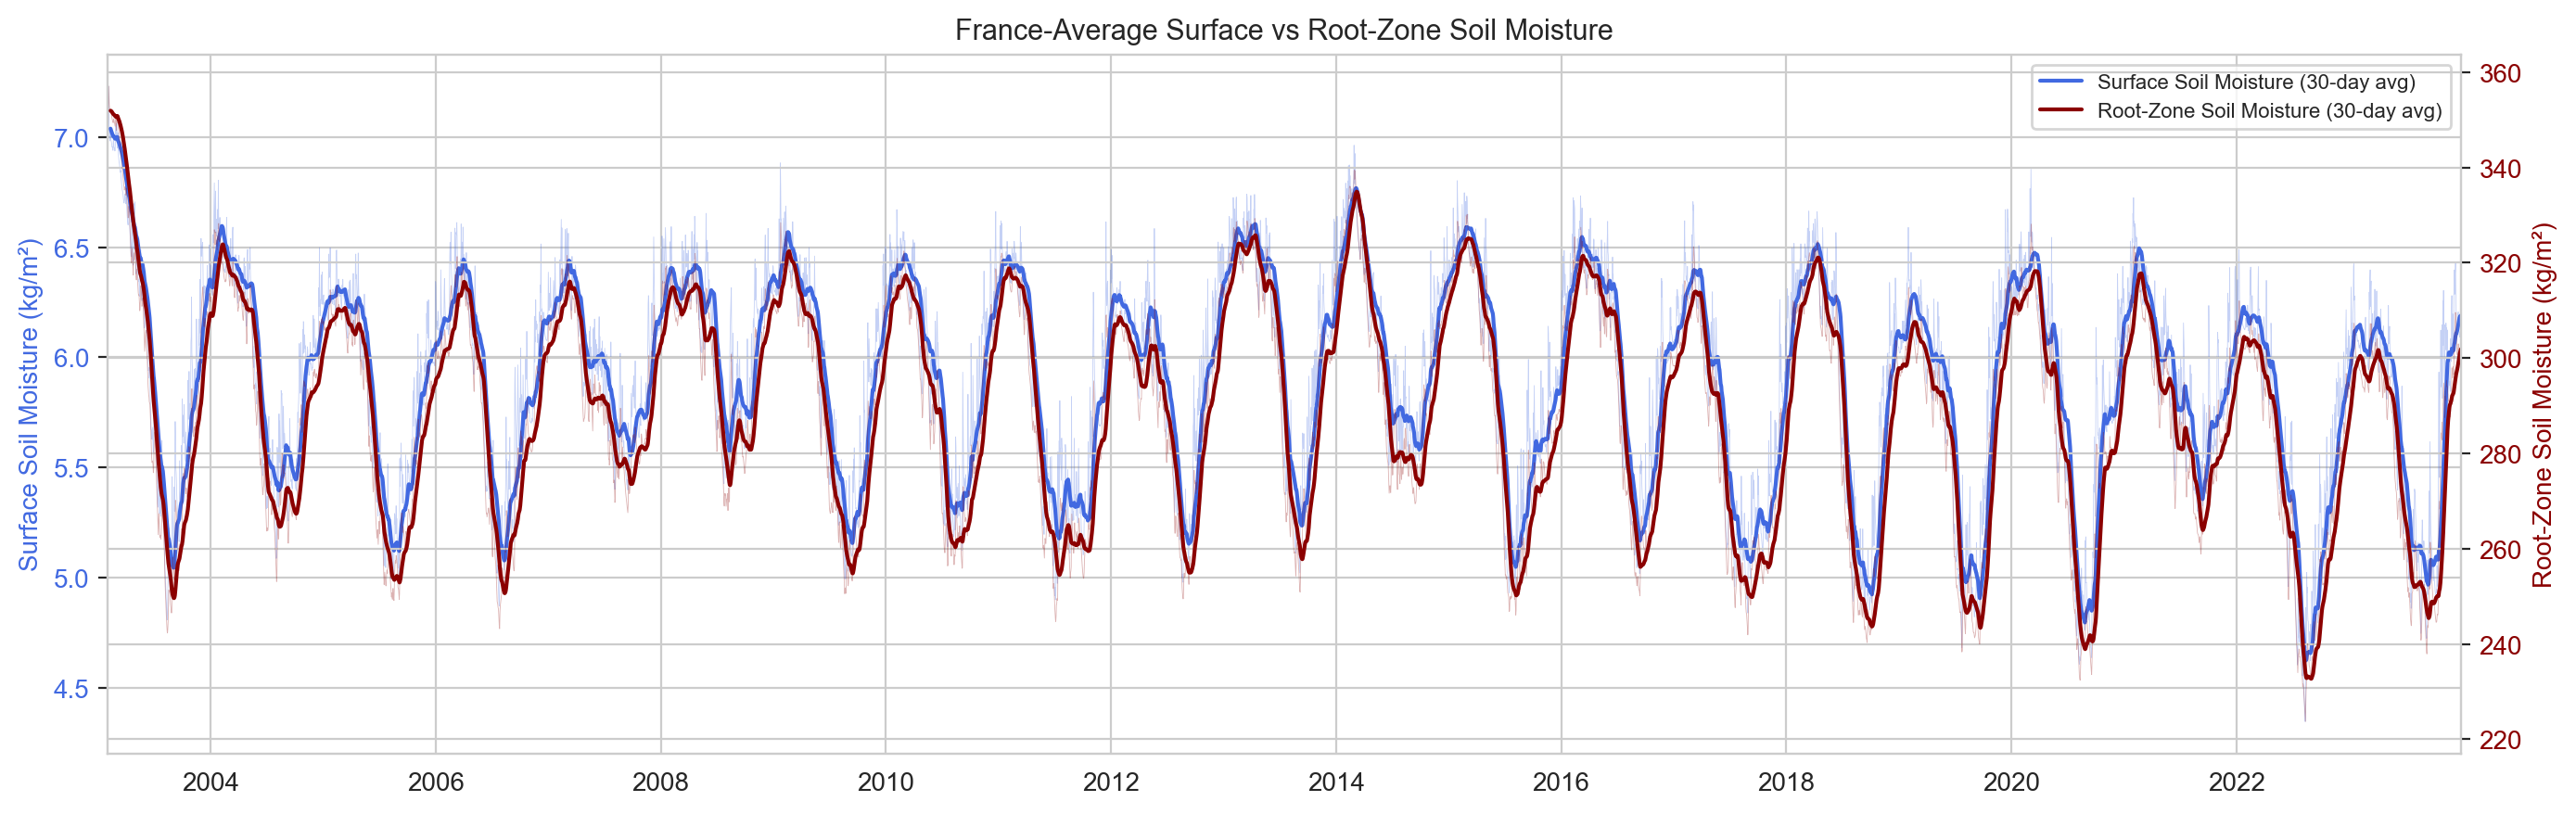
\includegraphics[width=\textwidth]{Figures/eda_soil_moisture.png}
    \caption{France-average surface soil moisture (blue, left axis) and root-zone soil moisture (red, right axis), 2003-2023. Surface moisture responds rapidly to individual precipitation events while root-zone moisture evolves more slowly, capturing different timescales of water availability despite near-perfect correlation ($r = 0.99$) in smoothed trends.}
    \label{fig:soil_moisture}
\end{figure}

\begin{figure}[ht]
    \centering
    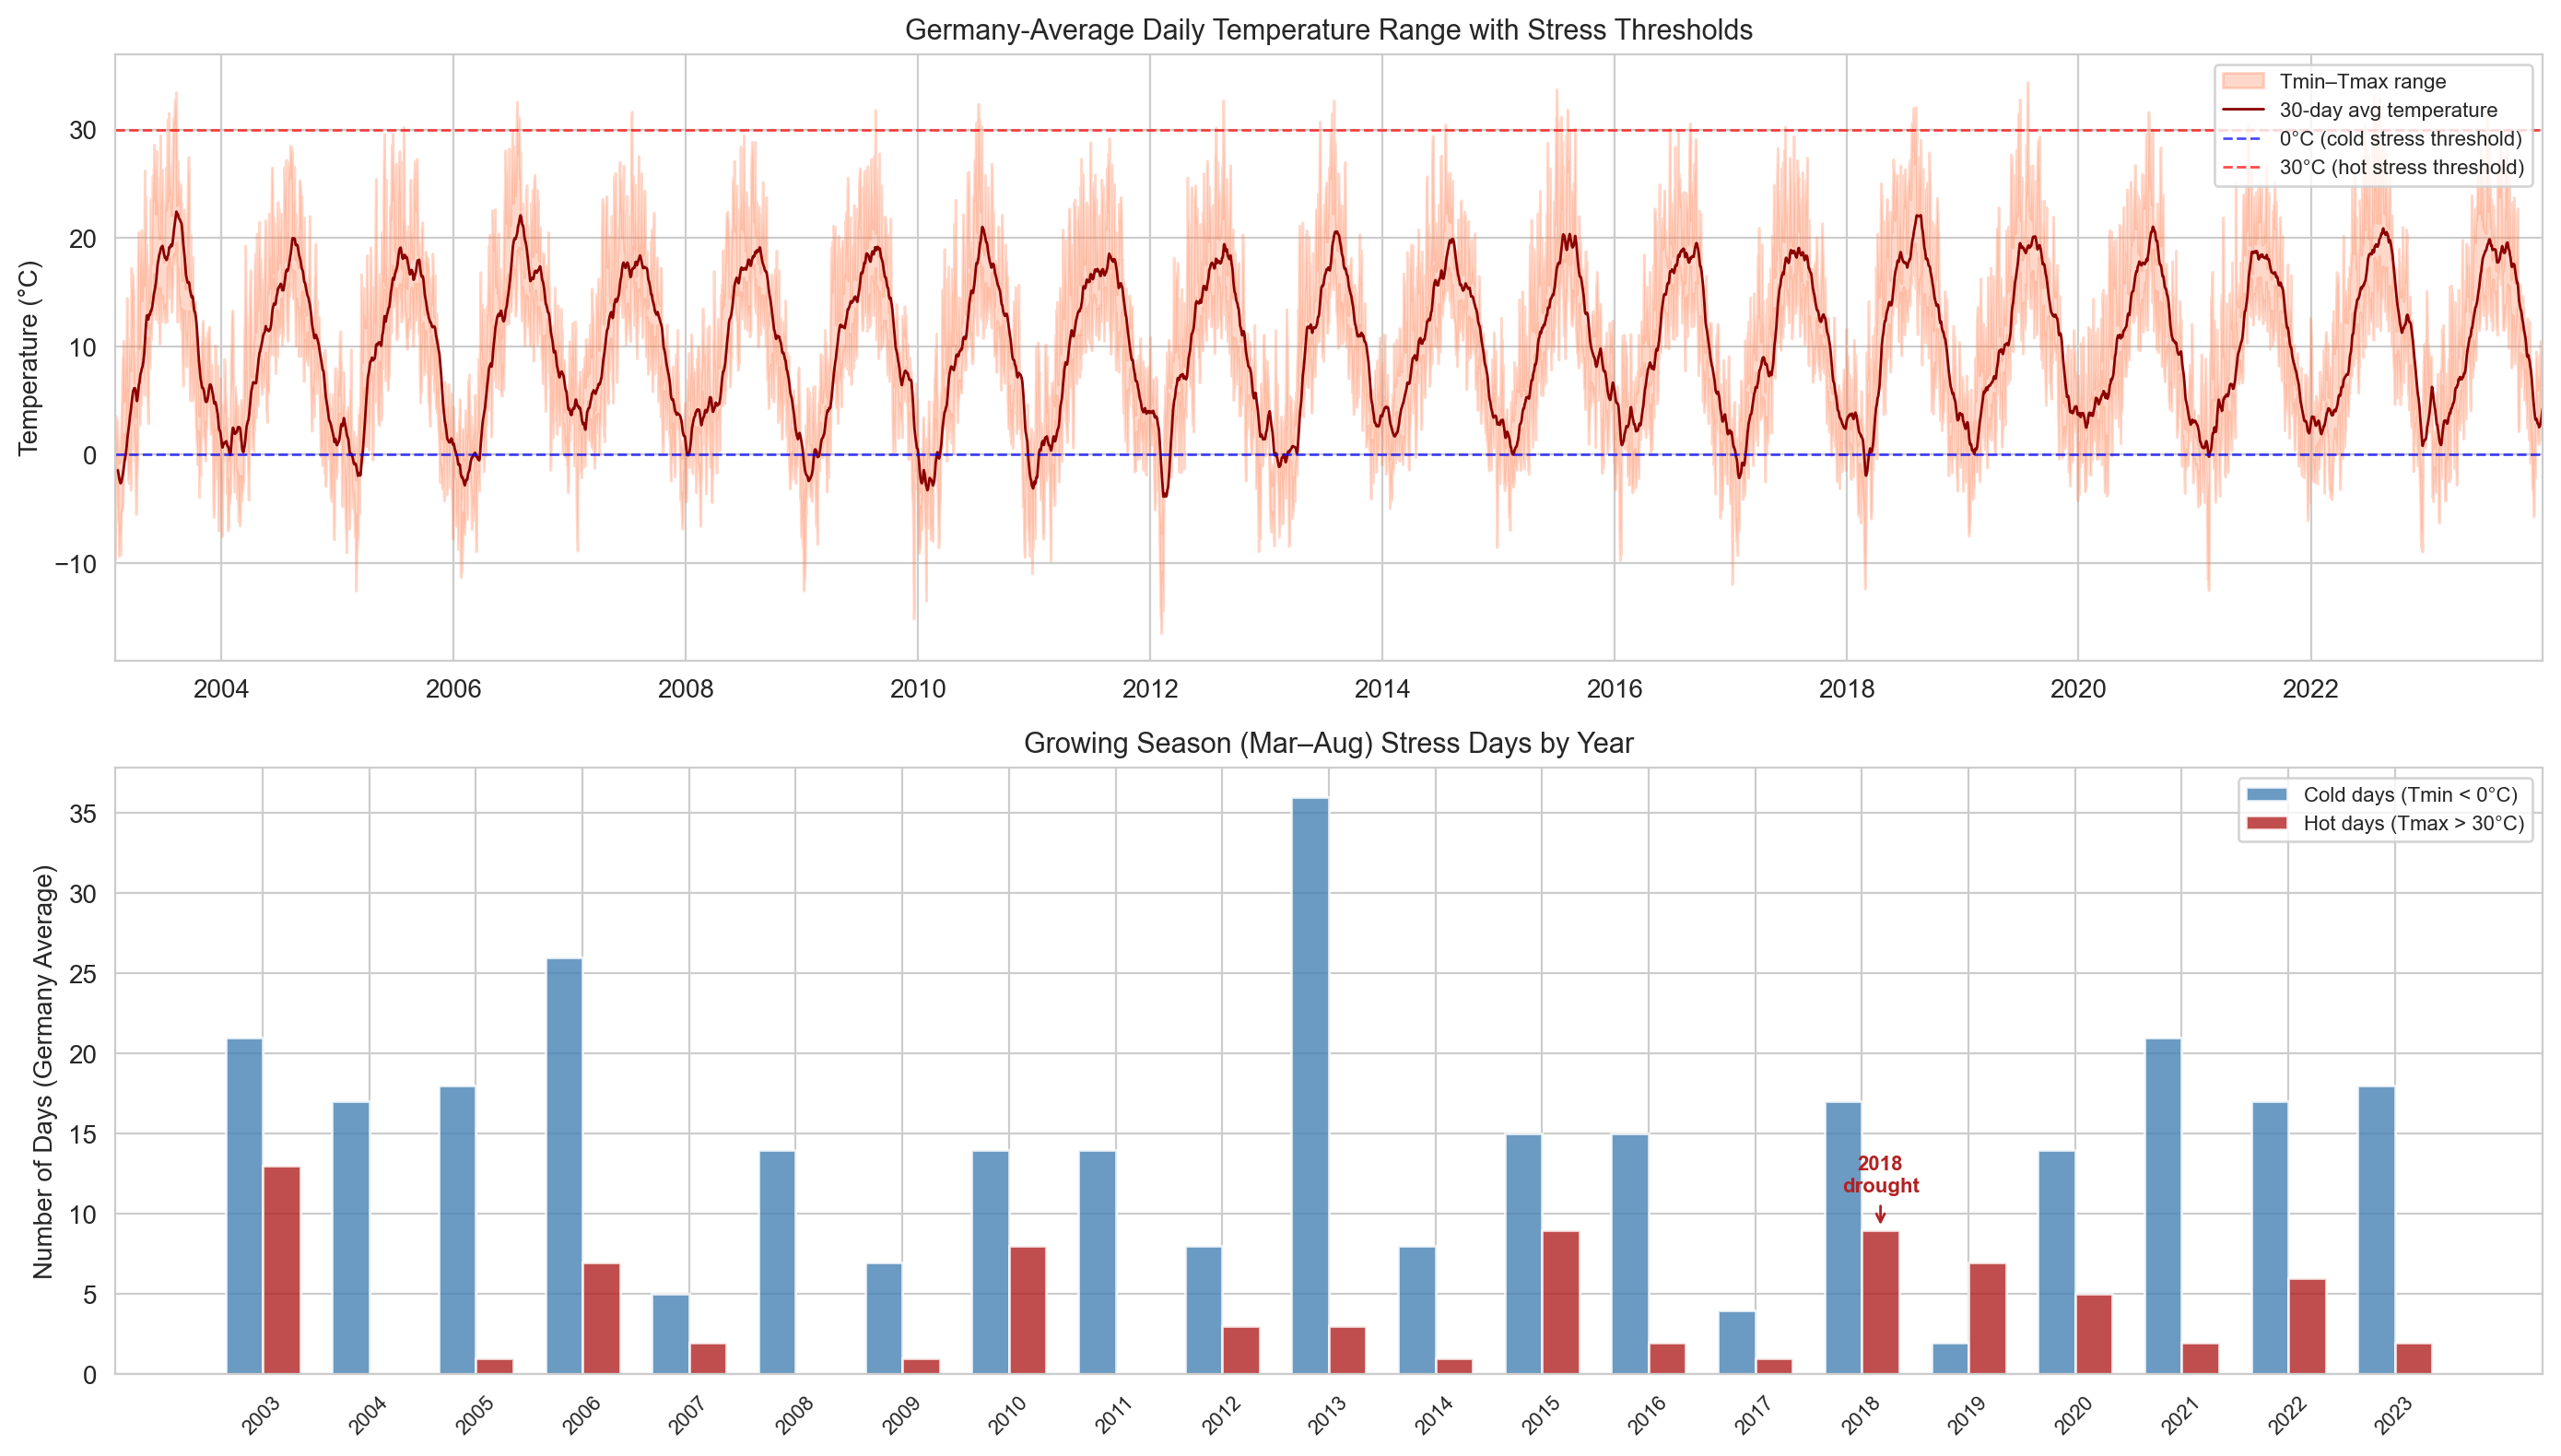
\includegraphics[width=\textwidth]{Figures/eda_temperature_stress_DE.png}
    \caption{Germany-average daily temperature range with stress thresholds (top) and annual growing-season (Mar-Aug) stress day counts (bottom). The 2018 European drought produced 2.5$\times$ the average number of hot stress days (Tmax $> 30$\textdegree C), motivating the threshold-based stress indicators in Section~\ref{sec:feature_eng}.}
    \label{fig:temp_stress_de}
\end{figure}

\begin{figure}[ht]
    \centering
    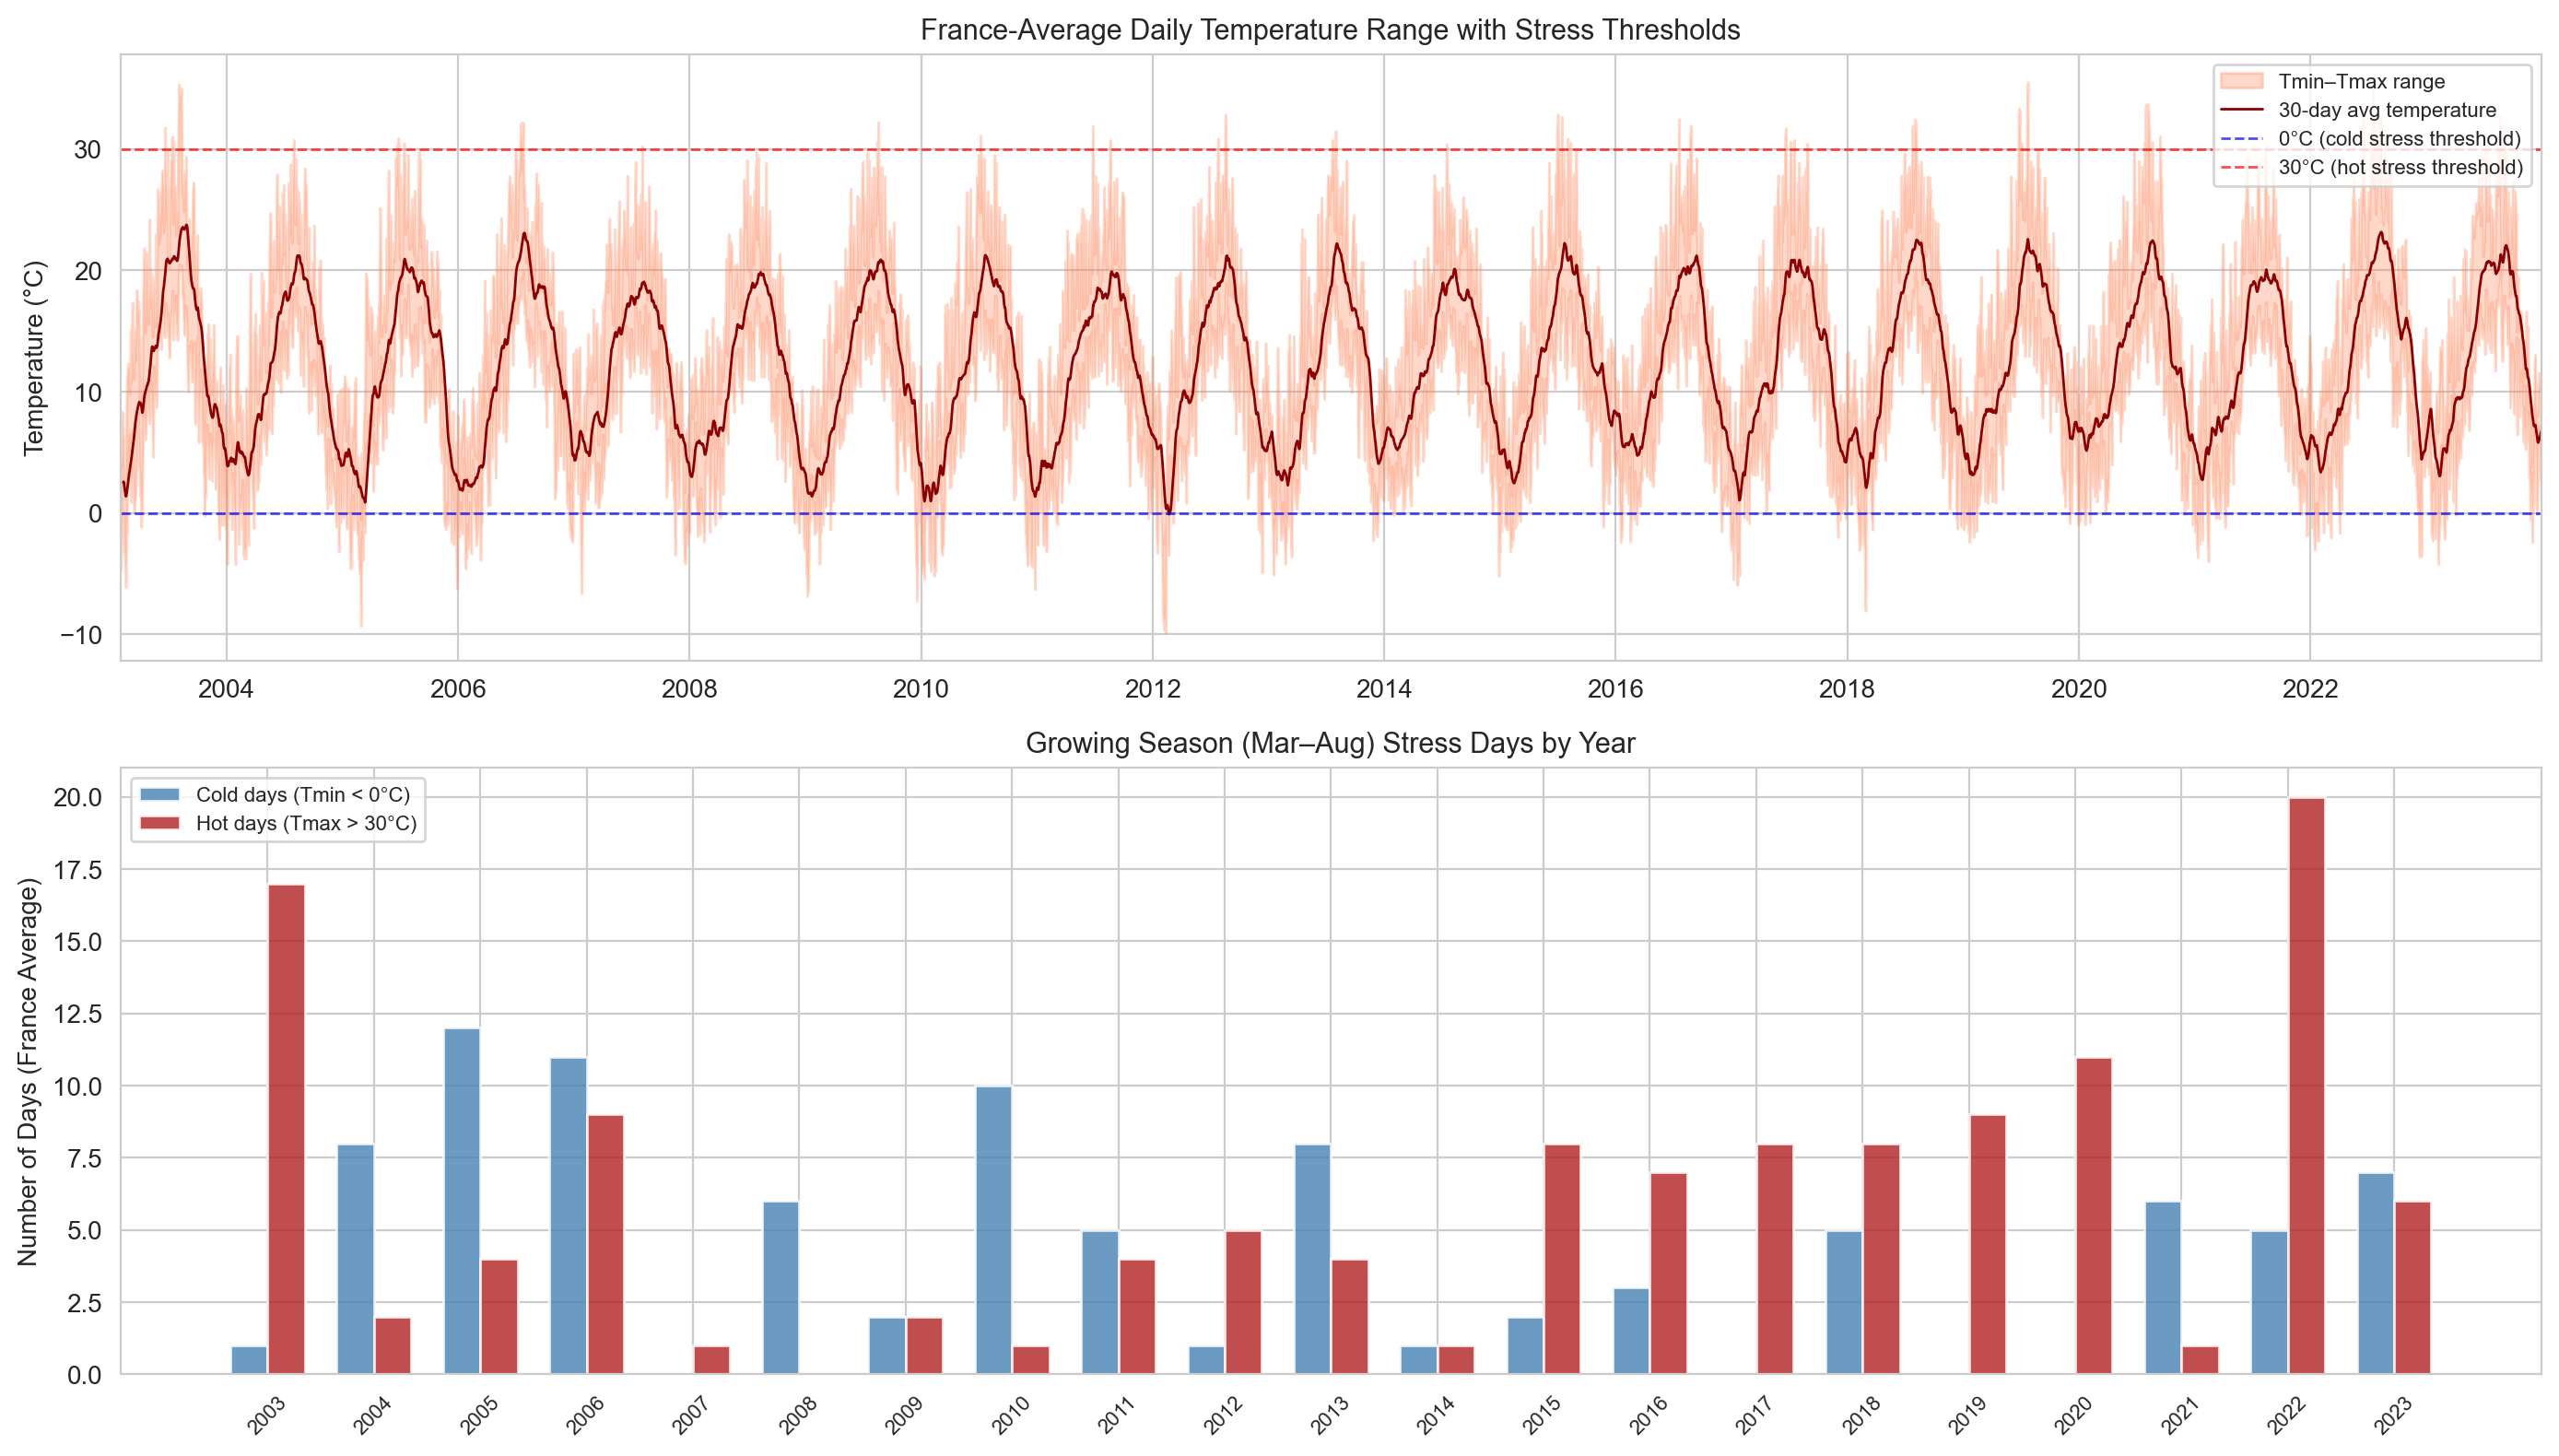
\includegraphics[width=\textwidth]{Figures/eda_temperature_stress_FR.png}
    \caption{France-average daily temperature range with stress thresholds (top) and annual growing-season stress day counts (bottom). France shows higher baseline hot-day frequency than Germany, with 2003 and 2022 as the most extreme heat years.}
    \label{fig:temp_stress_fr}
\end{figure}

\begin{figure}[ht]
    \centering
    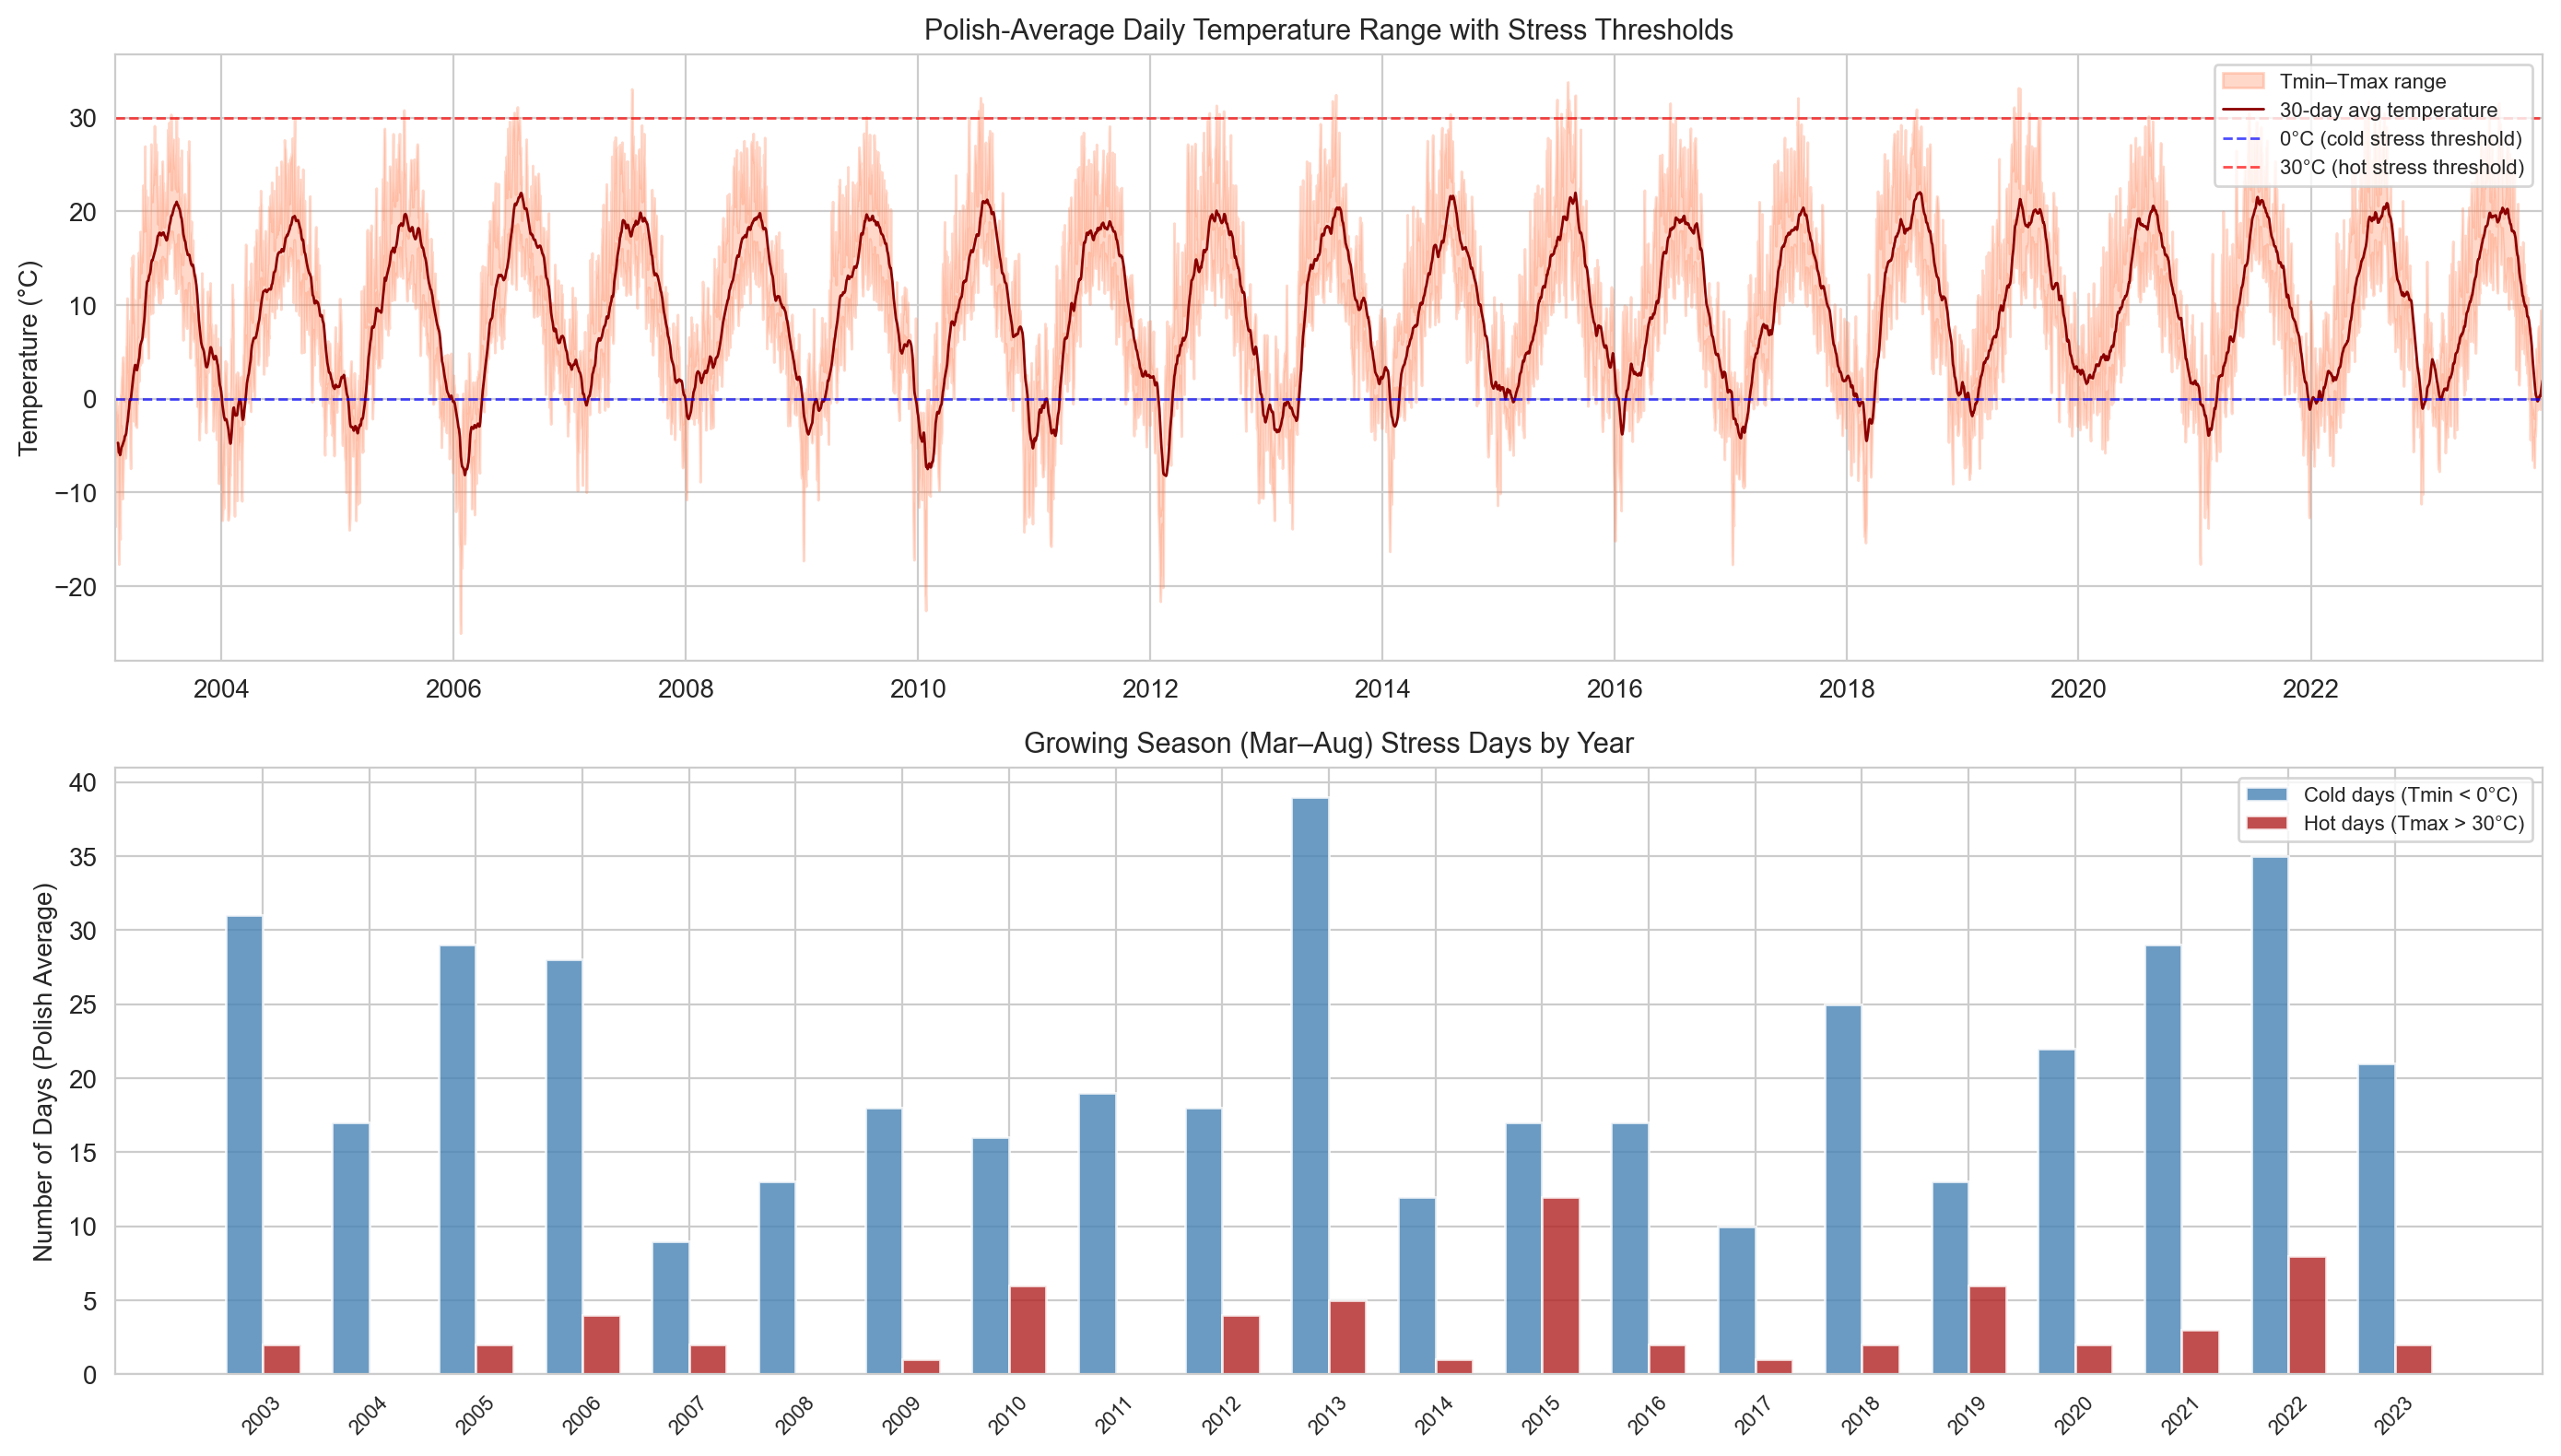
\includegraphics[width=\textwidth]{Figures/eda_temperature_stress_PL.png}
    \caption{Poland-average daily temperature range with stress thresholds (top) and annual growing-season stress day counts (bottom). Poland exhibits substantially more cold stress days than France or Germany, reflecting its continental climate, while hot stress events are comparatively rare.}
    \label{fig:temp_stress_pl}
\end{figure}

\begin{figure}[ht]
    \centering
    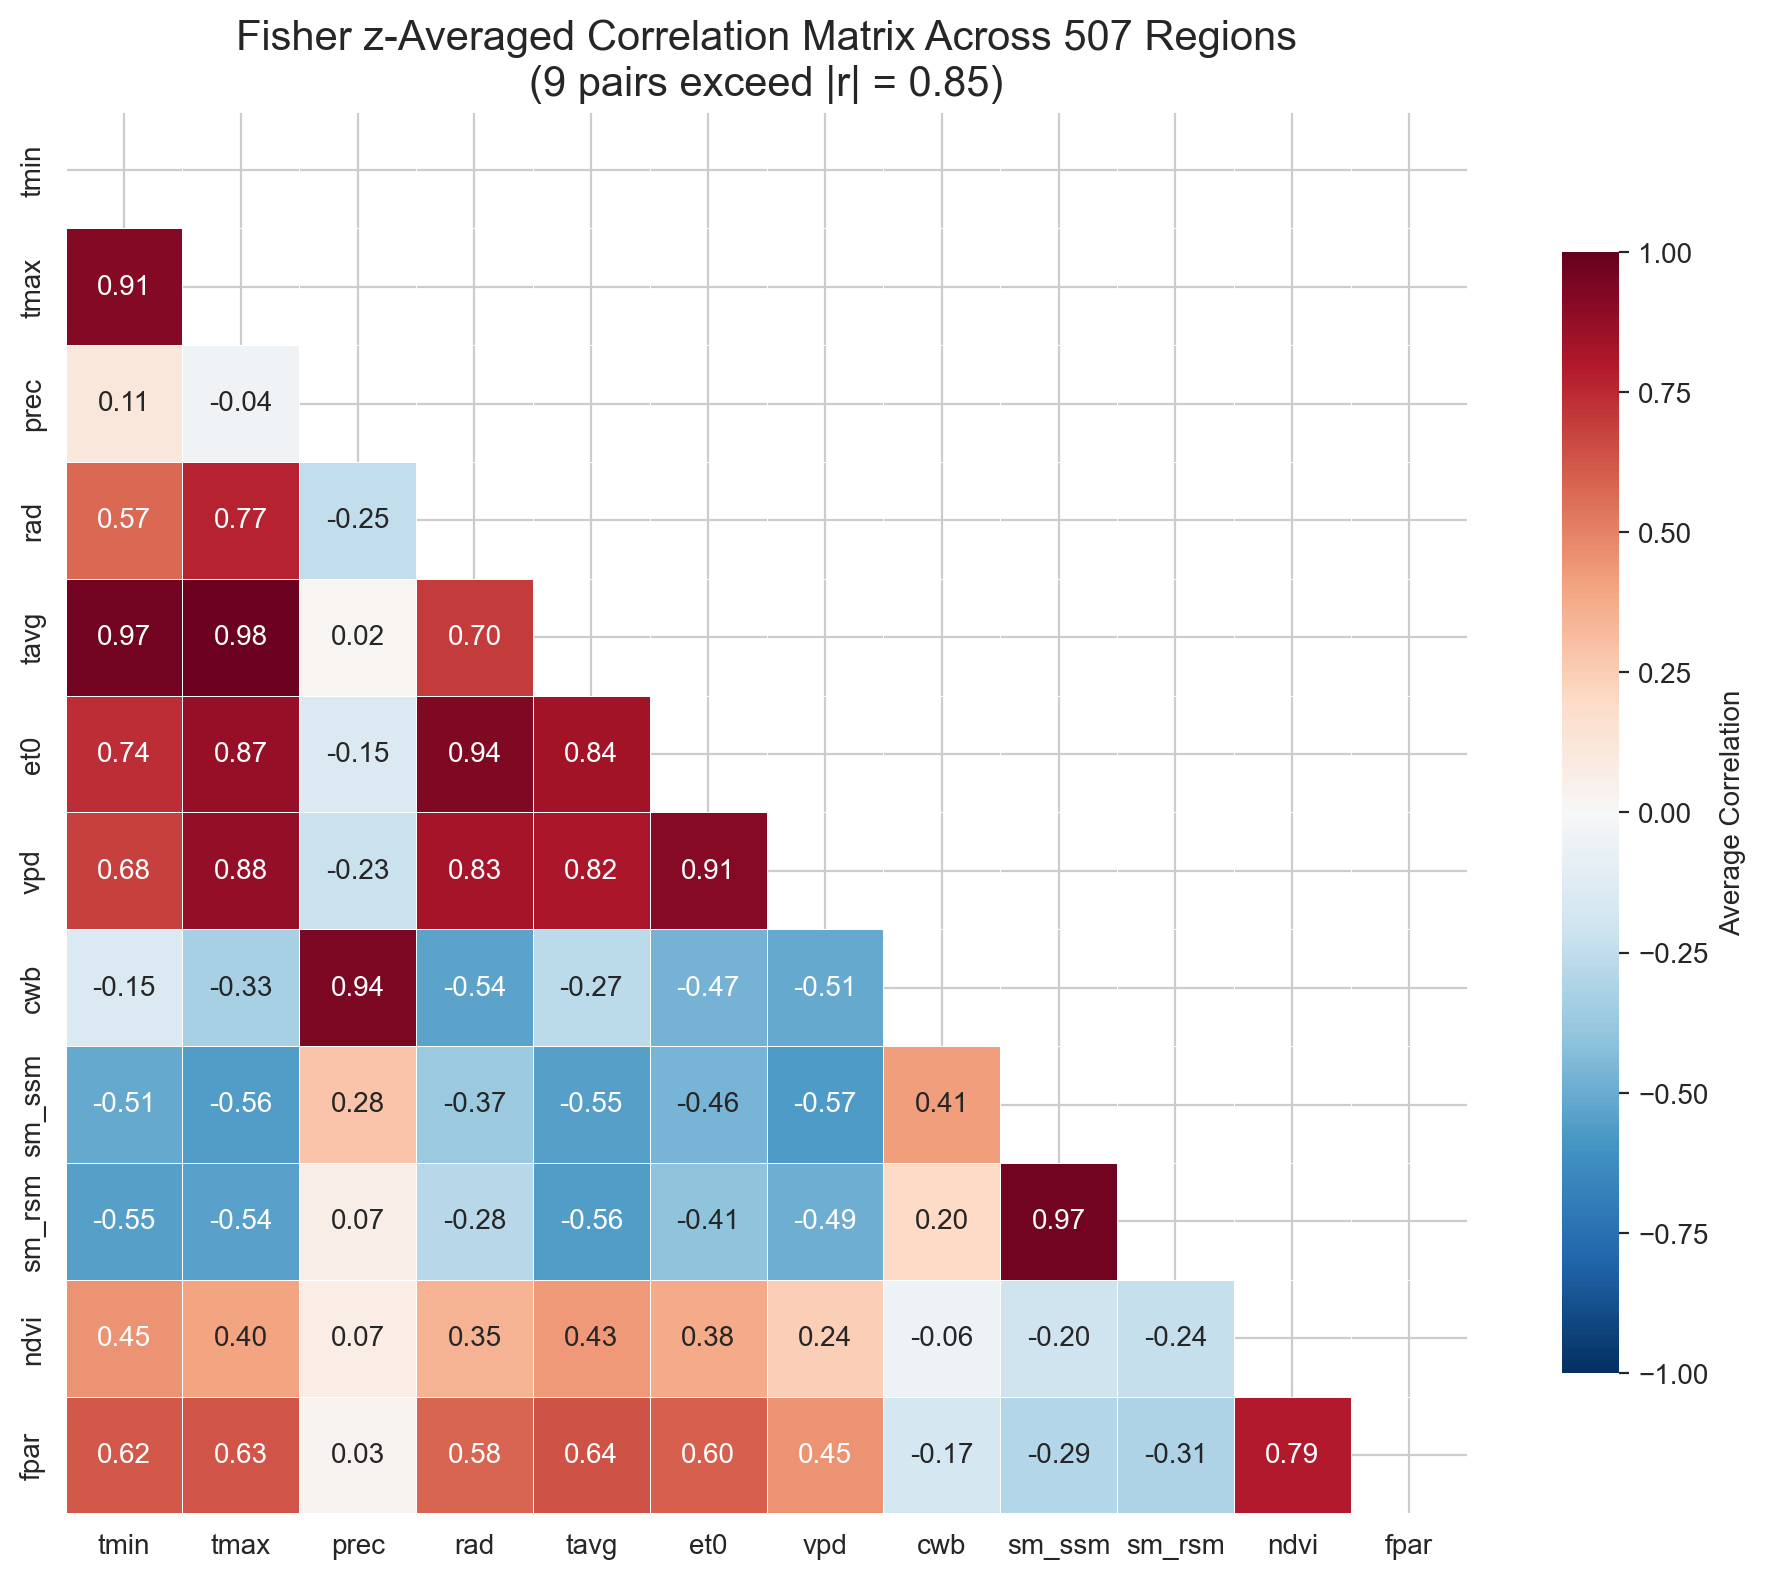
\includegraphics[width=0.75\textwidth]{Figures/eda_correlation_heatmap.png}
    \caption{Fisher z-averaged correlation matrix of the 12 raw CY-Bench variables across 507 regions. Nine feature pairs exceed $|\rho| = 0.85$, concentrated among temperature-derived variables. This motivates the correlation-based filtering applied before modelling.}
    \label{fig:corr_heatmap}
\end{figure}

\begin{figure}[ht]
    \centering
    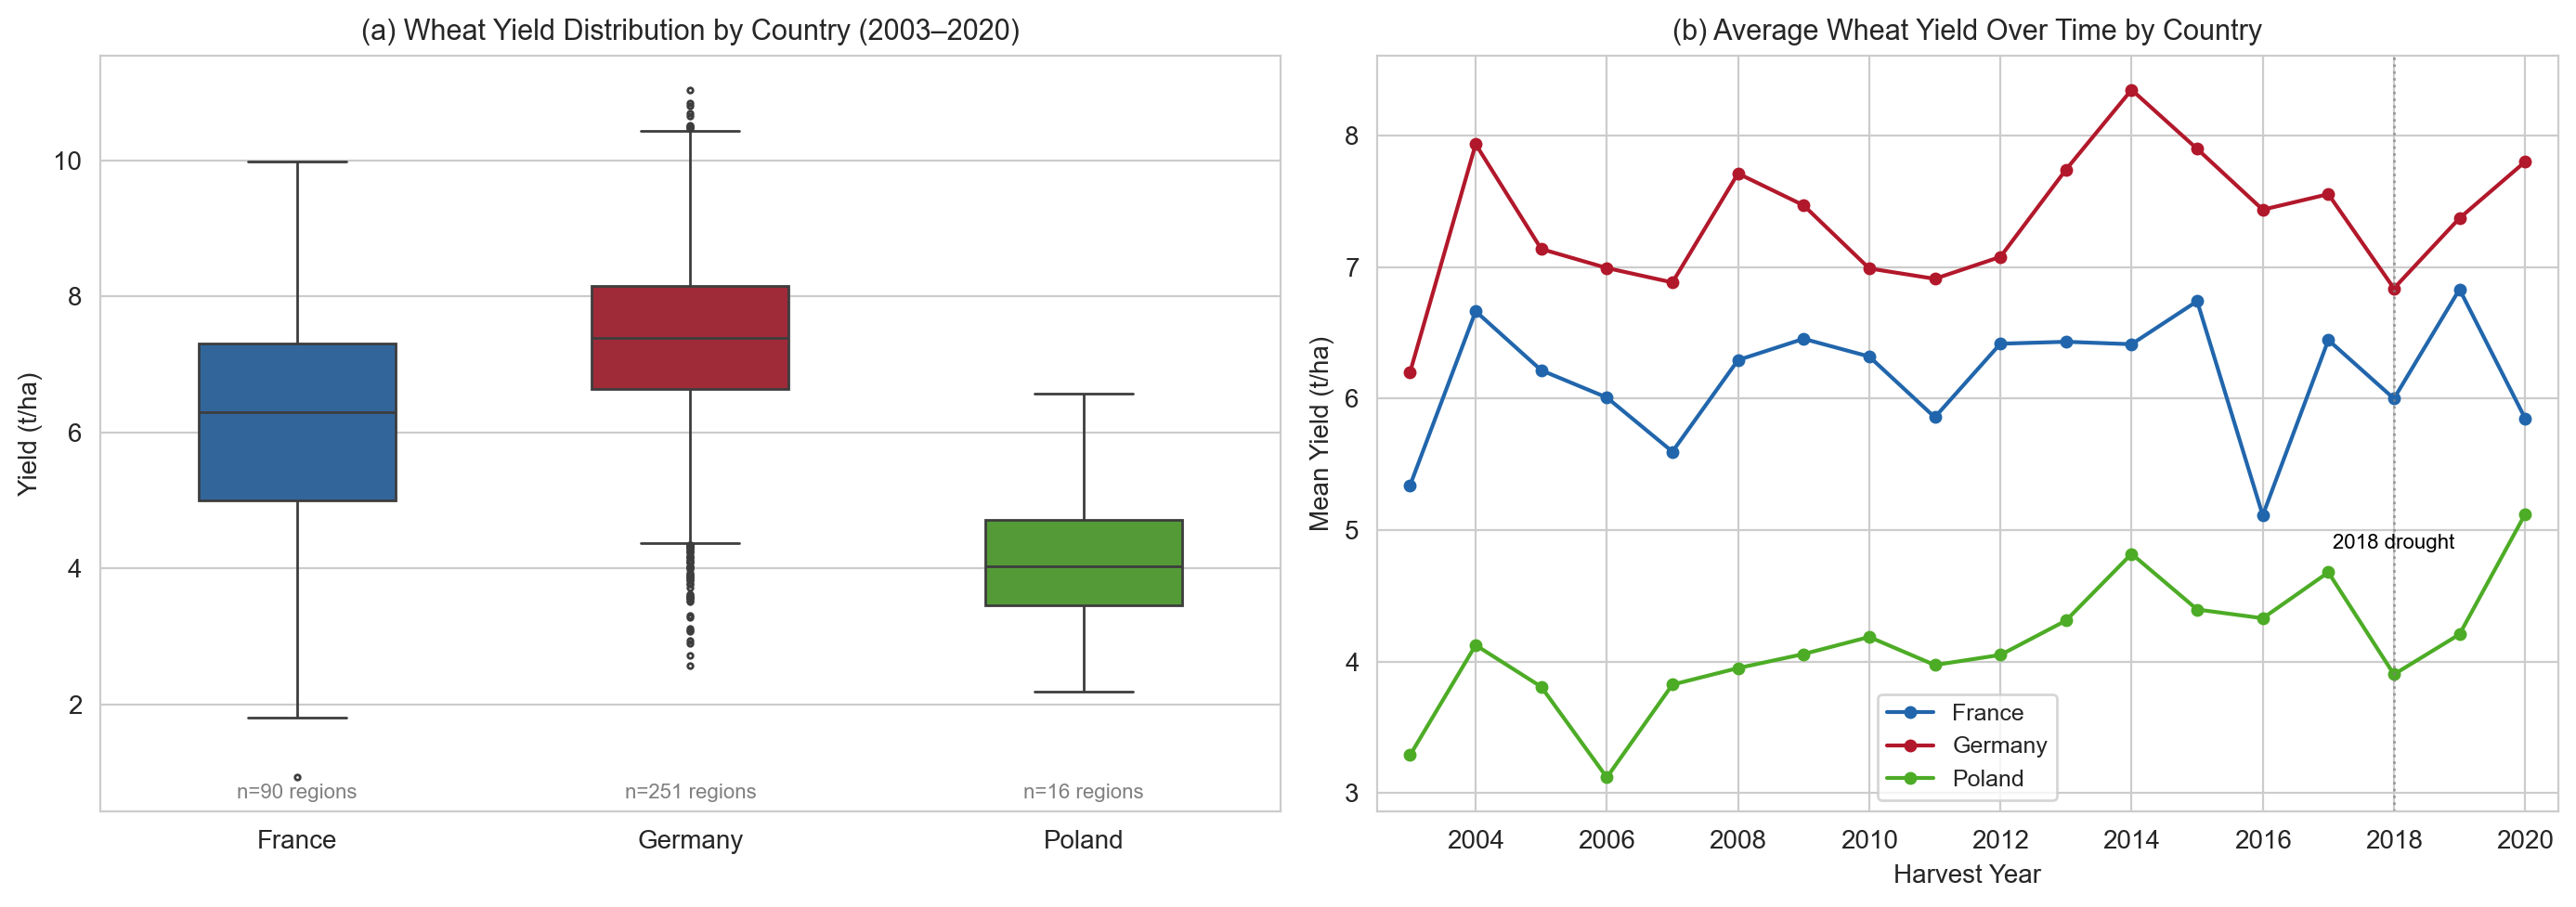
\includegraphics[width=\textwidth]{Figures/eda_yield_distributions.png}
    \caption{(a) Wheat yield distributions by country (2003-2020). Germany has the highest average yield (7.35 t/ha) and the widest spread across its 251 NUTS3 regions. (b) Average wheat yield over time by country. The 2018 European drought is visible as a synchronised dip, with Germany experiencing the largest decline ($-7.3\%$ relative to other years).}
    \label{fig:yield_dist}
\end{figure}

\section{Target Construction}\label{app:target_construction}

Apart from the timescale mismatch of daily returns and agricultural variables as well as the noise potentially present in returns at a daily scale, we also account for the fact that futures potentially have higher volatility once they approach expiration.

Indeed, the Samuelson hypothesis~\cite{bib54} predicts that futures price volatility increases as contracts approach expiration. Since we are looking at the closest maturing futures contract as our predictor, this implies that near-term price movements may display high variance. This further justifies our 5-day time window choice. Indeed, Duong and Kalev~\cite{bib55} tested this hypothesis in 20 futures markets and found strong support specifically for agricultural commodities. Daal et~al.~\cite{bib56} also confirm that the Samuelson effect is more pronounced for commodities rather than financial futures, however, they find the effect to be absent from most contracts they test. Overall, a weekly horizon enables us to reduce this higher-variance while remaining a short enough timeframe to be operationally relevant.

%%=============================================%%
%% For submissions to Nature Portfolio Journals %%
%% please use the heading ``Extended Data''.   %%
%%=============================================%%

%%=============================================================%%
%% Sample for another appendix section			       %%
%%=============================================================%%

%% \section{Example of another appendix section}\label{secA2}%
%% Appendices may be used for helpful, supporting or essential material that would otherwise 
%% clutter, break up or be distracting to the text. Appendices can consist of sections, figures, 
%% tables and equations etc.

\end{appendices}

%%===========================================================================================%%
%% If you are submitting to one of the Nature Portfolio journals, using the eJP submission   %%
%% system, please include the references within the manuscript file itself. You may do this  %%
%% by copying the reference list from your .bbl file, paste it into the main manuscript .tex %%
%% file, and delete the associated \verb+\bibliography+ commands.                            %%
%%===========================================================================================%%

\end{document}
